%-------------------------------------------------------------------------------
% IPOL LaTeX class manual
% by rafael grompone von gioi
% ver 0.5 - July 1, 2014
%-------------------------------------------------------------------------------
\documentclass{ipol}
\usepackage{mathrsfs} 

\usepackage{amsmath} 
\usepackage{amsfonts}
\usepackage{rotating} 
\usepackage{fancyvrb} 
%%for subfigure using ?
\usepackage{graphicx}
\usepackage{caption}
\usepackage{subcaption}
\usepackage{makeidx}
\usepackage{authblk}
\usepackage{algorithm}
\usepackage{algorithmic}  
\usepackage{amsthm}

\ipolSetTitle{Epipolar rectification of a generic camera  model}
\ipolSetAuthors{Marc Pierrot Deseilligny\ipolAuthorMark{1},
                Ewelina Rupnik\ipolAuthorMark{1}}
\ipolSetAffiliations{%
\ipolAuthorMark{1} LASTIG, Univ Gustave Eiffel, ENSG, IGN, F-94160 Saint-Mande, France\\
                   (\texttt{marc.pierrot-deseilligny@ensg.eu}, \texttt{ewelina.rupnik@ign.fr})
%\\\ipolAuthorMark{2} IIE, UdelaR, Uruguay (\texttt{jirafa@fing.edu.uy})
}

%---------------------------------------------
\newcommand{\CPP}{\mbox{\tt C\hspace{-0.05cm}\raisebox{0.2ex}{\small ++} }}
\newcommand{\SiftPP}{\mbox{\tt Sift\hspace{-0.05cm}\raisebox{0.2ex}{\small ++} }}



\newcommand{\RR}{\ensuremath{\mathbb{R}}}
\newcommand{\COM}[1]{}
\newcommand{\LA}{ LLLLLLLLLLLLLLLLLLLLLLLLLLLLLLLLLLLLLLLLLLLLLLLLLLLLLL \\ \\ }
\newcommand{\LALA}{ \LA \LA \LA \LA \LA \LA \LA \LA \LA \LA \LA \LA \LA \LA \LA  }


%// \newcommand{\HComp}{{}^{\longleftrightarrow}_{\pi_1,\pi_2}}
\newcommand{\HComp}{\overset{\Longleftrightarrow}{\scriptscriptstyle \pi_1,\pi_2}}
\newcommand{\PiOT}[1]{\pi_1(\pi_2^{-1}(#1))}
\newcommand{\PiTO}[1]{\pi_2(\pi_1^{-1}(#1))}
\newcommand{\CurvO}{{\mathcal{T}_1}}

%  Bundles
\newcommand{\Bund}[1]{\ensuremath{\mathcal{B}_{#1}}}
\newcommand{\BundO}{\Bund{1}}
\newcommand{\BundT}{\Bund{2}}
\newcommand{\BundK}{\Bund{k}}


% Epipolar lines
\newcommand{\LineE}[1]{\ensuremath{\mathcal{L}_{#1}}}
\newcommand{\LineO}{\LineE{1}}
\newcommand{\LineT}{\LineE{2}}
\newcommand{\LineK}{\LineE{k}}

\newcommand{\CurveE}[1]{\ensuremath{\mathcal{C}_{#1}}}
\newcommand{\CurveO}{\CurveE{1}}
\newcommand{\CurveT}{\CurveE{2}}
\newcommand{\CurveK}{\CurveE{k}}

% "Epipolar Surface"
\newcommand{\Sv}{\ensuremath{\mathcal{S}_{v}}}

\newcommand{\BigV}[1]{\ensuremath{\overrightarrow{#1}}}
\newcommand{\TanO}[1]{\BigV{t_1#1}}
\newcommand{\TanT}[1]{\BigV{t_2#1}}

\newcommand{\Negl}[1]{\ensuremath{\mathcal{O}(#1)}}



\newcommand{\PiVert}{\widetilde{\pi}}
%\newcommand{\PiOT}{\Pi^{12}}
%\newcommand{\PiTO}{\Pi_{2\rightarrow 1}}

\newcommand{\DerPart}[2]{\frac{\partial #1}{\partial #2}}

\newtheorem{theorem}{Theorem}
\newtheorem{notation}{Notation}
\newtheorem{definition}{Definition}
\newtheorem{remark}{Remark}

\definecolor{orange}{rgb}{1,0.5,0} 
\newcommand{\er}[1]{\textcolor{orange}{#1}} 

%-------------------------------------------------------------------------------
\begin{document}

%-------------------------------------------------------------------------------
\begin{ipolAbstract}
ble
\end{ipolAbstract}

%-------------------------------------------------------------------------------
\ipolKeywords{epipolar rectification, generic camera}

%-------------------------------------------------------------------------------
\section{Introduction}
Epipolar geometry of images plays a central role in many applications in the field of photogrammetry and computer vision. Within the stereo-reconstruction pipeline, it intervenes twice:

\begin{enumerate}
   \item In the camera pose orientation step when computing the
      relative orientation of a pair images from their corresponding points. Assuming the projection follows the central perspective and the internal calibration is known, one can compute the epipolar geometry using the essential matrix.
   \item In the image dense matching step where the epipolar rectification simplifies the correspondence search because we know
        that for a point $(x_1,y)$ in image $I_1$, its correspondence is some point
        $(x_2,y)$ in image $I_2$. Therefore, finding correspondences across images reduces to a $1$ dimensional problem.
\end{enumerate}

\noindent In this paper, we only study  the epipolar rectification problem and more specifically
its application to a generic camera model, focusing on the pushbroom sensors.

\subsection{Related works}
Rectifying a pinhole camera stereo pair comes down to transforming their original epipolar geometry to a canonical form where: (a) their focal planes are coplanar, (b) their conjugate epipolar lines are colinear, and (c) parallel to the camera's x-axis. 
%It is equivalent of sending the stereo pair's epipoles at infinity. 
From the algebraic standpoint, it is equal to applying two 2D projective transformation to either images of the stereo pair. Several approaches to compute such transformations have been proposed over the course of the last 30 years. For a calibrated stereo pair (i.e. with known camera projection matrices), there exists a unique rectifying transformation, up to a rotation along the baseline~\cite{fusiello2000epi}. In an uncalibrated case, the solution is obtained by factoring out two 2D homographies from the fundamental matrix. Because there are no two unique homographies, the common practice is to parametrize these transformations such that the distortions caused by rectifying are minimized. For instance, Loop and Zhang~\cite{loop1999epi} decompose the rectifying homographies to a combination of the projective, similarity, shearing transforms and impose that the first stays close to an affine mapping. Hartley~\cite{hartley1999epi} satisfies a condition that for a neighborhood of a point (e.g. the center of an image) the computed homography is a rigid transformation. Building on this work, Isgro and Trucco's~\cite{isgro1999epi} approach obtains a unique solution by minimizing the x-disparity, without having to explicitly calculate the fundamental matrix. Instead of minimizing the disparity in the first coordinate, Wu and Yu~\cite{wu2005epi} recycle an idea first introduced by Hartley~\cite{hartley1999epi} which requires that the aspect ratio of the images before and after rectification is constant. More recently, Fusiello and Irsara~\cite{fusiello2008epi} introduced the camera matrices back into the equation and proposed a \textit{quasi}-Euclidean approach for uncalibrated cameras, similar to that of the calibrated cameras case. Their projective transformations are parametrized by five angles and a focal length. Monasse \textit{et al.}~\cite{monasse2010epi} break down the one-time rotation of~\cite{fusiello2008epi} to a three step procedure, and prove increased robustness by using a geometric error measure (i.e., camera rotation angle) to reduce the rectifying error distortions.

%force the plane at infinity to be close to the plane at infinity of a calibrated stereo pair. This is possible by making an educated guess and estimating only the focal length.


 
%Epipolar recitification algorithms for central projection cameras can be classified into calibrated and uncalibrated camera approches.


%For central projection cameras, the epipolar recitification algorithms are grouped into the calibrated and uncalibrated camera case. Rectifying calibrated cameras comes down to fixing their perspective center and rotating the cameras until their focal planes are coplanar (Fusiello compact algo). Uncalibrated camera rectification involve additional parameters 

  
%
Unlike the central projection camera model, pushbroom-like sensors acquire each image row from a different perspective center. As a consequence, the epipolar lines are neither straight lines, nor are they conjugate across the image~\cite{Gupta1997}.  One way to overcome this particularity is to simplify the projection function with a 2D affine~\cite{ono1999epipolar,wang2011epipolar} or a parallel projection model~\cite{morgan2006epipolar}. Such approximations usually come at a prize of the loss of precision, especially with the increasing camera field-of-view or in mountainous scenes. In the context of image dense matching, de~Francis \textit{et al.}~\cite{deFrancis2014stereo} improves the precision by partitioning the images into small patches for which indepedent affine rectifictions are computed. Alternatively and with equally good precision, Oh~\cite{Oh2011} uses the \textit{Rational polynomial coefficients} (RPCs) to map the epipolar curves across the full size images with lines in a piecewise approach.
%
%ù while being locally approximated to straight lines. Oh~\cite{Oh2011} approximates the epipolar curves of an image pair by piecewise linear curves with a set of virtual correspondences. An image pair is then resampled to an equivalent geometry, imposing that the conjugate curves become straight and aligned on the y-axis. 


%uses the \textit{Rational polynomial coefficients} (RPCs) to trace the epipolar curves across image pairs with a dense set of virtual correspondences, and by doing so approximates the curves by a piecewise linear curve. Given a set of correspondences, an image pair is then resampled to an equivalent geometry, imposing that the conjugate curves become straight and aligned on the y-axis. 

%This work is similar to the approch proposed by Oh~\cite{Oh2011} in that it tries to model the epipolar curves across the entire image at once.
 
%  \cite{wang2011epipolar}

%The x-parallax remains linearly proportional to the depth of corresponding points - yes because we don(t move the x-coordinates

 
%\cite{orfeo2008}

%Carlo de Franchis , split the images in small patch, in each patch compute a coniq camera that approximate the model for each pair, make an epipolar resampling of this approximate coniq camera.  Advantage : simple an reuse existing method. Drawback : need small patch to be accurate enough.

%\begin{itemize}
   %\item Isabelle Veillet :   these a l'IGN bureau Lahman
 %  \item Ooh \cite{Oh2011}  : par suivi de ligne  
 %  \item orientation by epipolar (Samantha )
%\end{itemize}

NOUS: 
\begin{itemize}
\item nous optimization global donc repartition d'erreur (Oh no)
\item no a priori on narrow FOV, altitude diffs in terr wrt the satellite altitude (true for affine approximations) 
\item no need for localisation model (true for all except for Wang?)
\end{itemize}

%\subsection{Topic of the paper}



\section{The mathematics of epipolar geometry in the generic case}

\subsection{Formalisation and notation of projections}

\begin{figure}
\centering
\begin{tabular}{||c||}
 \hline \hline
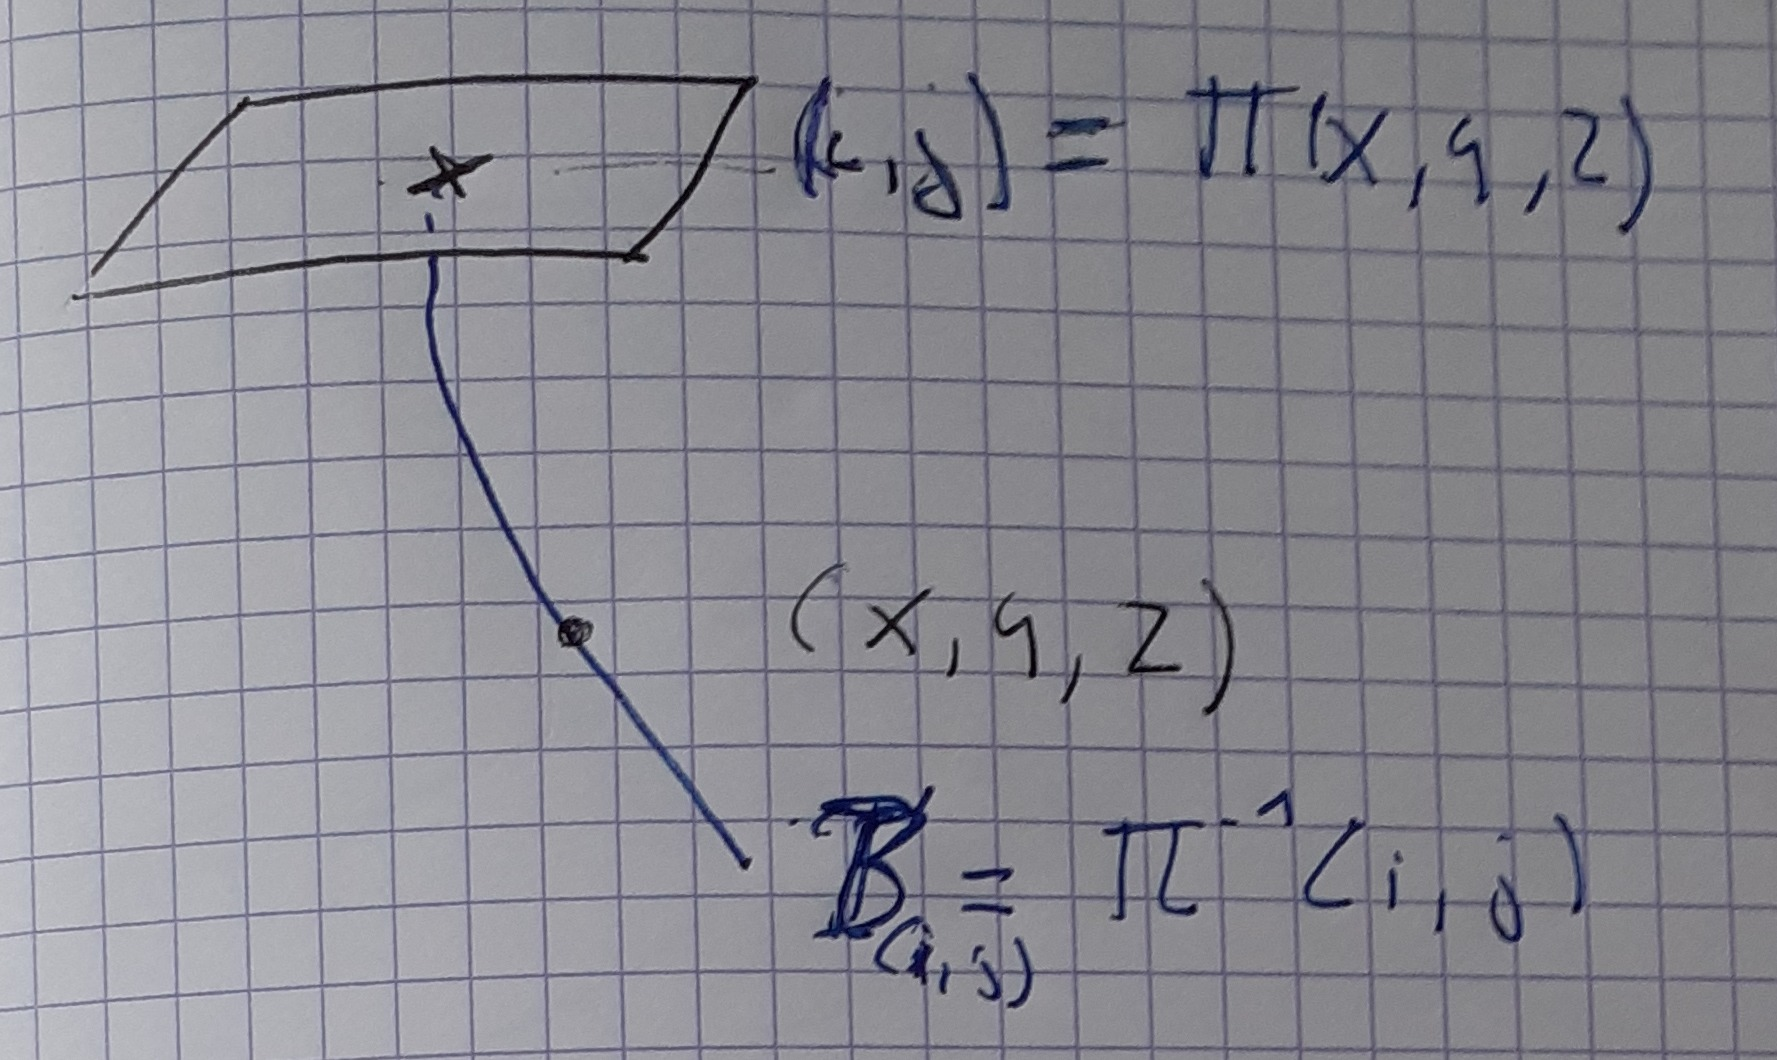
\includegraphics[width=10cm]{FIGS/NotaProj.jpg} 
 \\ \hline \hline
\end{tabular}
\caption{A projection and a bundle}
\label{FigNotaProj}
\end{figure}



%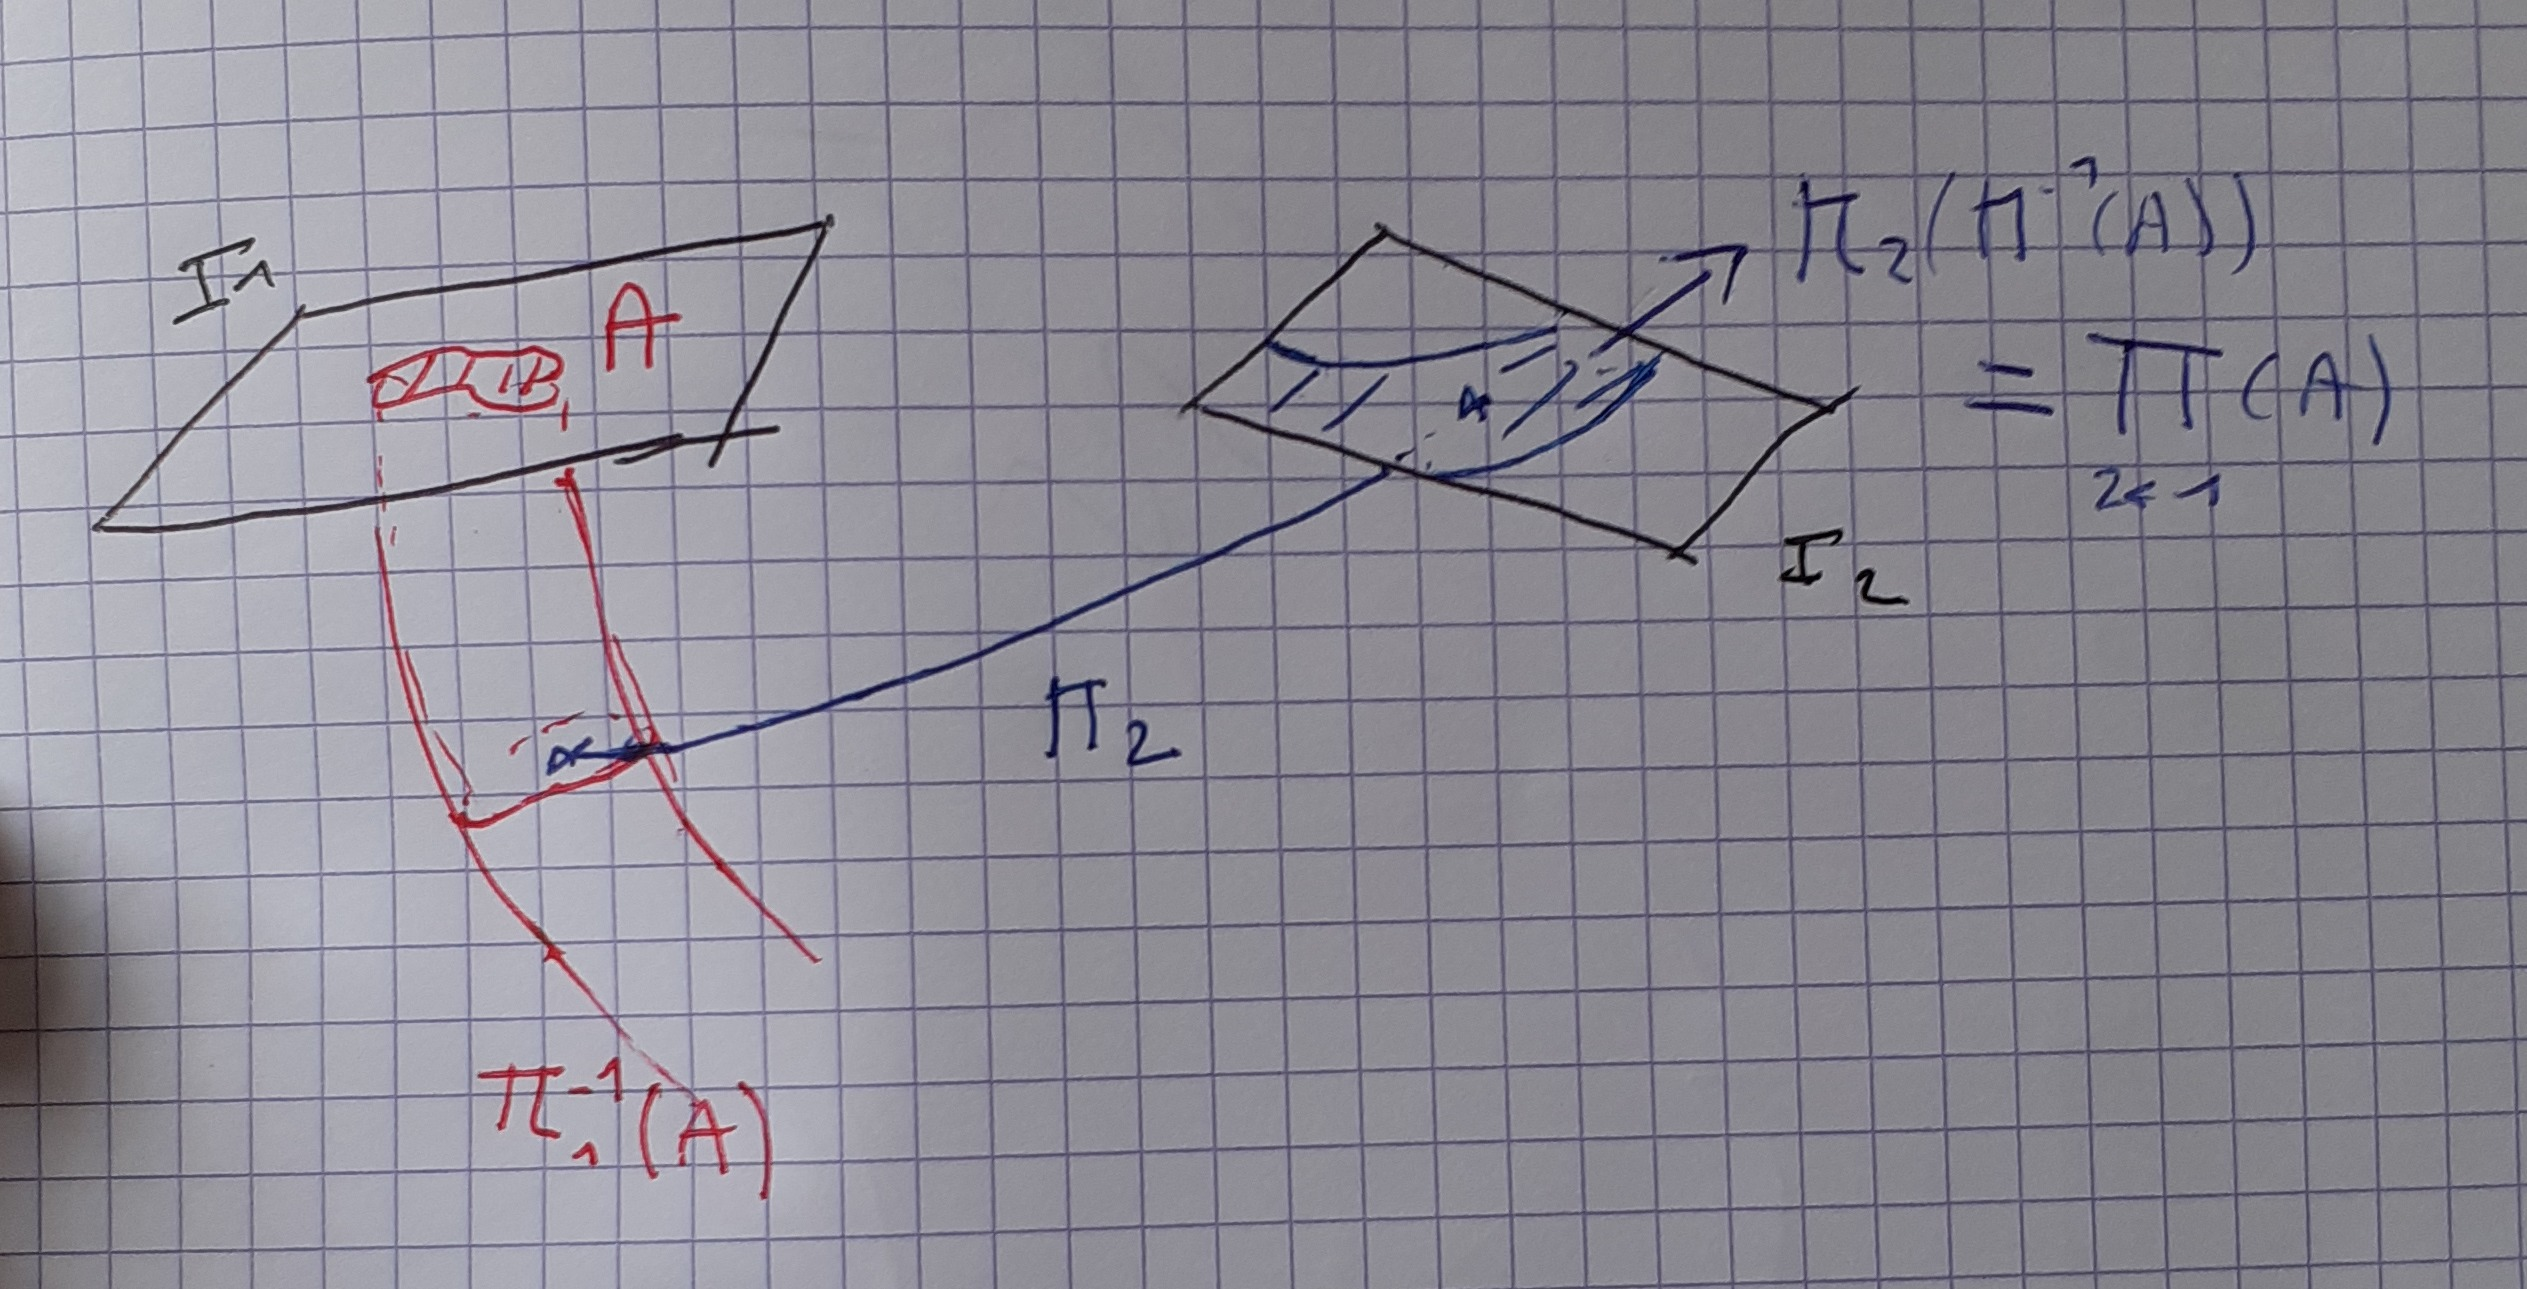
\includegraphics[width=12cm]{FIGS/NotaSets.jpg}

We define the geometric sensor model of an image by a projection function $\pi$, that computes for a given 3D
point its 2D projection in the image:

\begin{definition}[Generic geometric sensor model]  

\emph{Illustrated in Figure~\ref{FigNotaProj}.}

A geometric sensor model $\pi$ is a $\mathcal{C}^{\infty}$ mapping from ground space $(\RR^3)$ to image space $(\RR^2)$:

\begin{equation}
  \pi :  \RR^3  \rightarrow \RR^2  ,  (X,Y,Z)  \rightarrow (i,j) = \pi(X,Y,Z). \label{Eq:Proj}
\end{equation}
\end{definition}

\noindent Next, we define the bundles of a projection :

\begin{definition}[Bundle]
For $p_k \in I_k$ we note $\BundK(p_k)$  the bundle corresponding to $\pi_k^{-1}(p_k)$. \er{When there is no confusion},
we note identically  $\BundK(P)$, where $P\in \RR^3$,
 the bundle corresponding to $\pi_k^{-1}(\pi_k(P)) = \BundK(\pi_k(P))$.
\end{definition}


\noindent Later, for simplicity we will use the  {quasi vertical} hypothesis, which allows to extend $\pi$ to a
bijective mapping of $\RR^3$ and compute its inverse:

\begin{definition}[Quasi vertical camera model]  
We say that the projection is quasi vertical if the following mapping $\PiVert$ is a diffeomophism of $\RR^3$:
\begin{equation}
  \PiVert :  \RR^3  \rightarrow \RR^3  ,  (X,Y,Z)  \rightarrow (i,j,Z) = \PiVert(X,Y,Z)  , with (i,j) = \pi(X,Y,Z). \label{PiInvert}
\end{equation}
\end{definition}

\noindent Given $2$ images $I_1$ and $I_2$, the knowledge  of their geometric models $\pi_1$ and  $\pi_2$
reduces the matching between $2$ images to a 1D problem. In fact, given a point $p_1$ in $I_1$,
we can compute the 3D curve $\BundO(p_1)$ of  ground points that project to $p_1$ in $I_1$, and compute its
homologous curve in $I_2$ with $\pi_2(\BundO(p_1))$. We now define the H-compatible relation between two points
by the following definition:

\begin{definition}[H-Compatible, $\HComp$] 
\emph{Illustrated on Figure~\ref{FigNotaComp}.}

We says that $p_1$ in  $I_1$ and $p_2$ in $I_2$ are  $\pi_1-\pi_2$ H-compatible, and write $p_1 \HComp p_2$, if   the following condition is satisfied:

\begin{equation}
   ( \BundO(p_1) \cap  \BundT(p_2) \neq \emptyset    )
    \Leftrightarrow
  (\exists P \in  \RR^3 : \pi_1(P) =p_1 ,  \pi_2(P) = p_2).
\end{equation}
\end{definition}

\begin{figure}
\centering
\begin{tabular}{||c||}
 \hline \hline
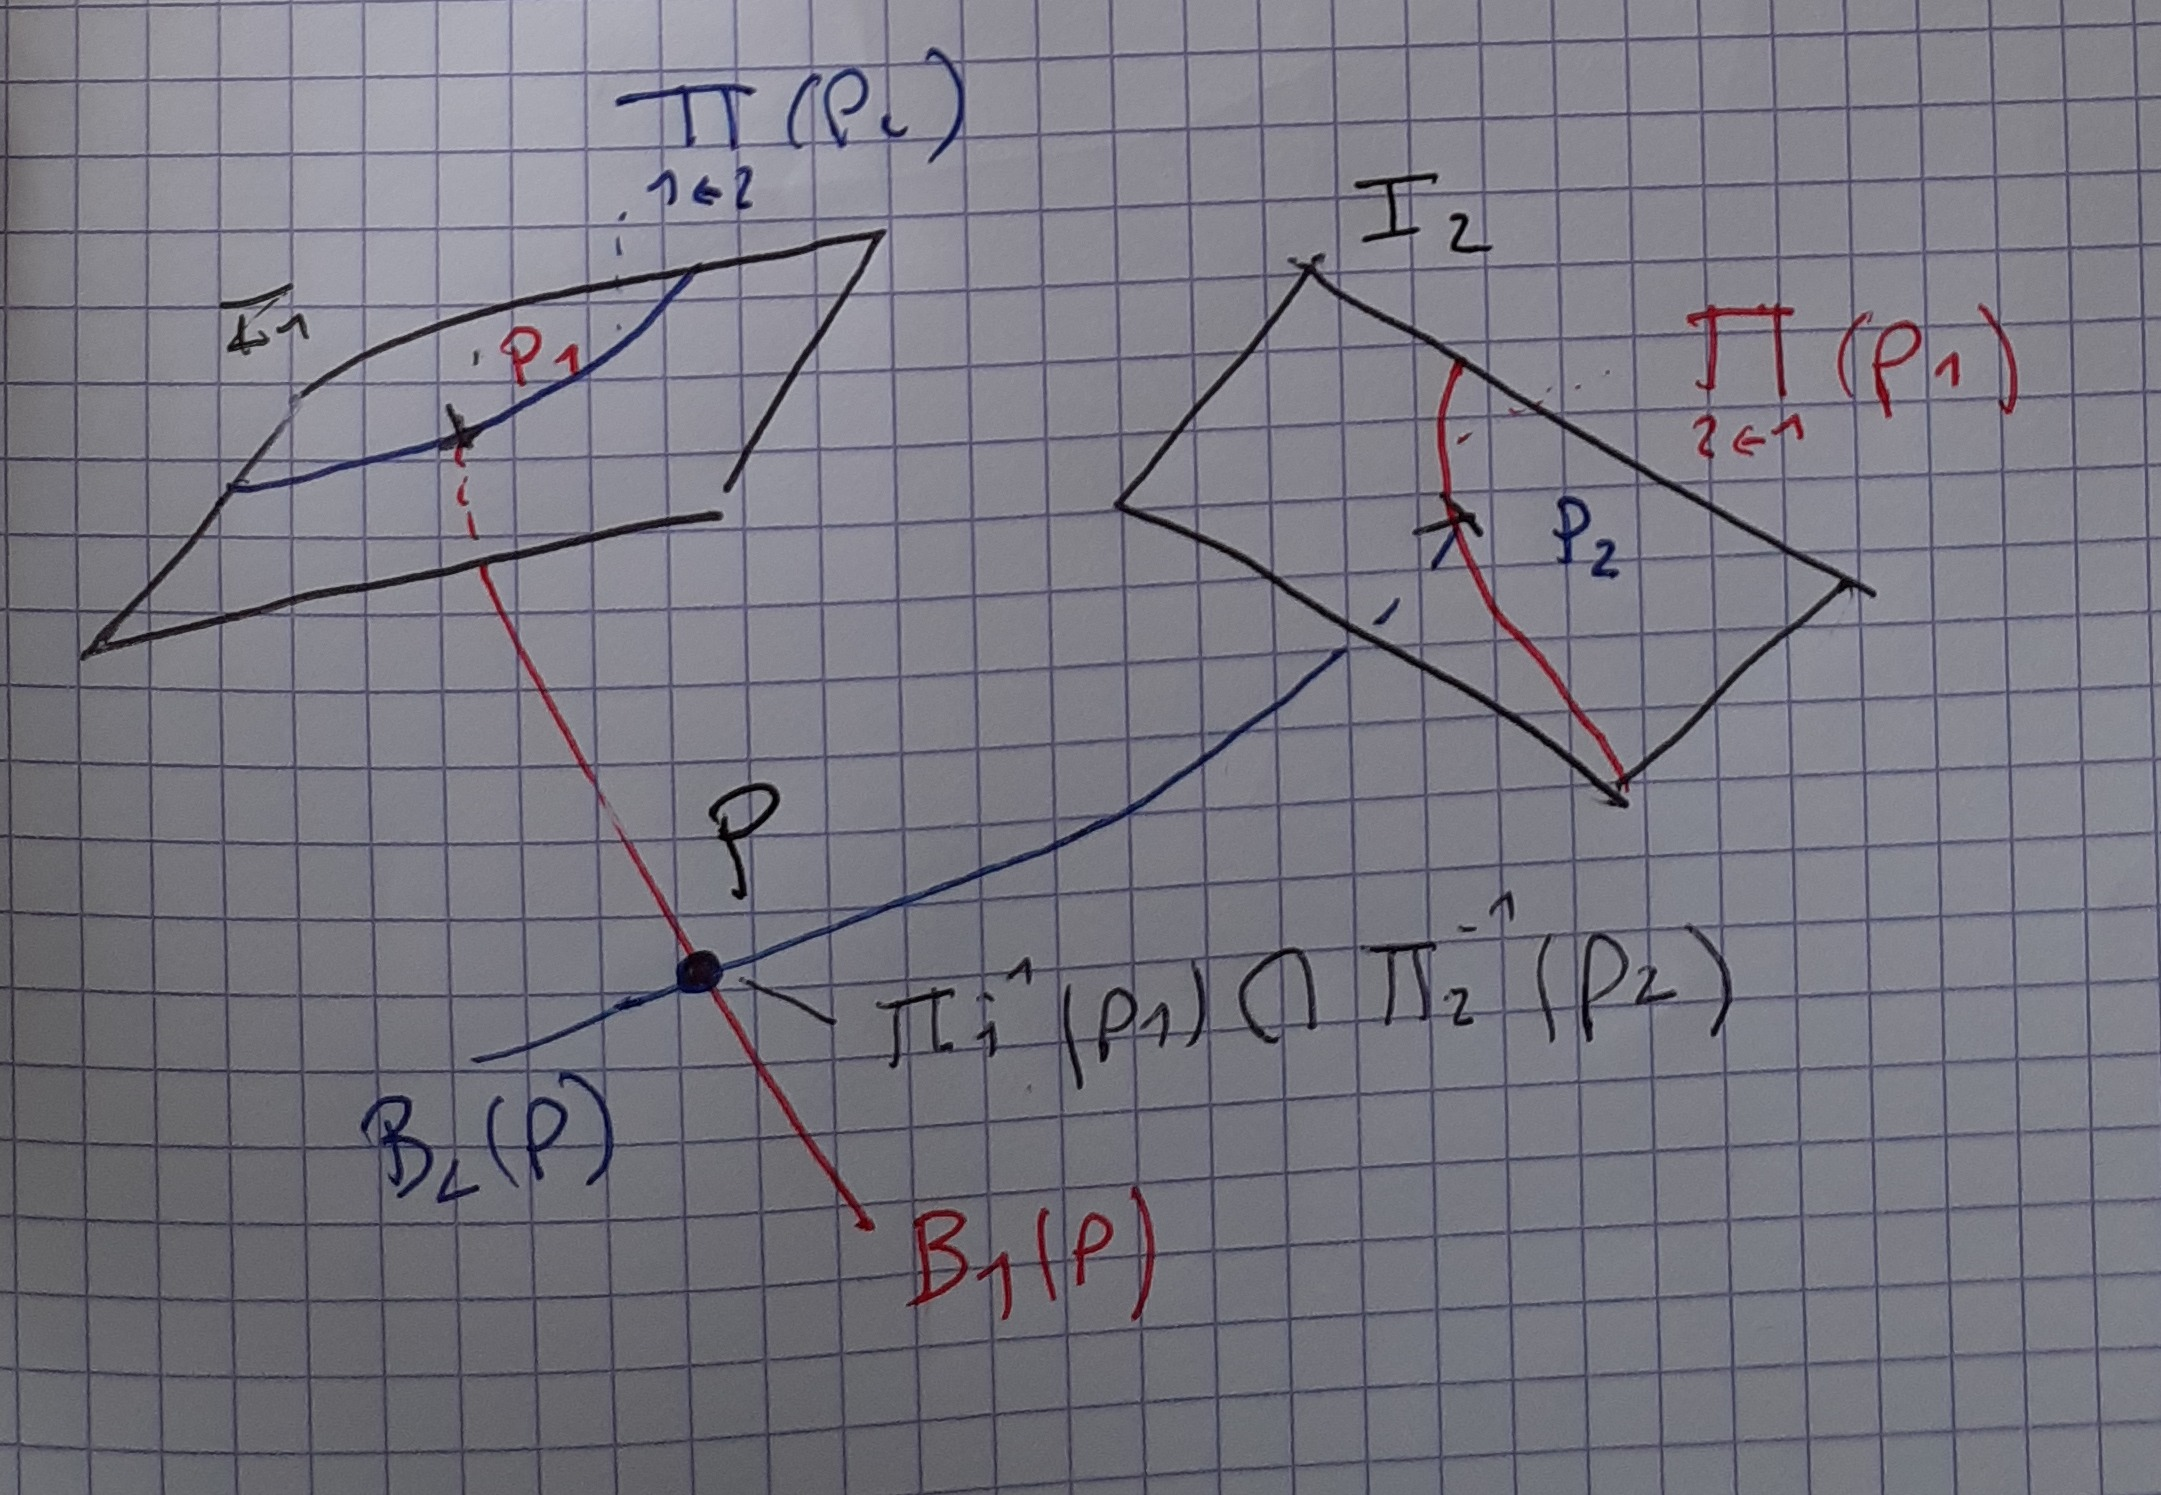
\includegraphics[width=15cm]{FIGS/NotaBundle.jpg} 
 \\ \hline \hline
\end{tabular}
\caption{Illustration of $\HComp$}
\label{FigNotaComp}
\end{figure}

\noindent In image matching, the relation $p_1 \HComp p_2$  means that $p_1$ and $p_2$ are potentially homologous.

%---------------------------------------------
%---------------------------------------------
%---------------------------------------------



% - - - - - - - - - - - - - - -
\subsection{Definition of epipolar geometry}

In fact, the previous relations are sufficient to implement all the matching techniques and
$(\pi_1,\pi_2)$ can be used to define a matching process taking advantage
of the~\emph{a priori} knowledge on the scene geometry. That is, given a point in one image, we can easily
follow its curve of potentially homologous points in the other image.
This way of handling geometry (i.e., without the epipolar geometry) has also the advantage of being adaptable to multi-image matching. We can thus see that epipolar geometry is not required in the image matching process.

The drawback of this approach is that it mixes, in the same routine, two 
different problems: the handling of the geometry and resampling on one side;
the matching process on the other side. When one is interested
in matching of a single image pair, the epipolar geometry
can provide an "elegant" solution to separating the problem in two independent problems. \er{ER thinks this should be removed $\rightarrow$} When two images are in epipolar geometry, two points $p_1,p_2$ are potential homologous iff they have the same ordinate ($y_1=y_2$).

\begin{definition}[Epipolar Geometry]
\emph{Illustrated in Figures~\ref{FigDefEpip} and~\ref{FigAmbigEpip}.}

Let $\pi_1,\pi_2$ be two cameras and let $\phi_1,\phi_2$  be two diffeomorphisms
of $\RR^2$. We say that $\phi_1,\phi_2$ are epipolar resamplings iff:

\begin{equation}
  \forall e_1=(u_1,v_1) , e_2=(u_2,v_2) : (v_1=v_2)   \Leftrightarrow  (\phi_1^{-1}(e_1) \HComp \phi_2^{-1}(e_2)).
\end{equation}
   \label{EqEpiEgalY}
\end{definition}

\begin{figure}
\centering
\begin{tabular}{||c||}
 \hline \hline
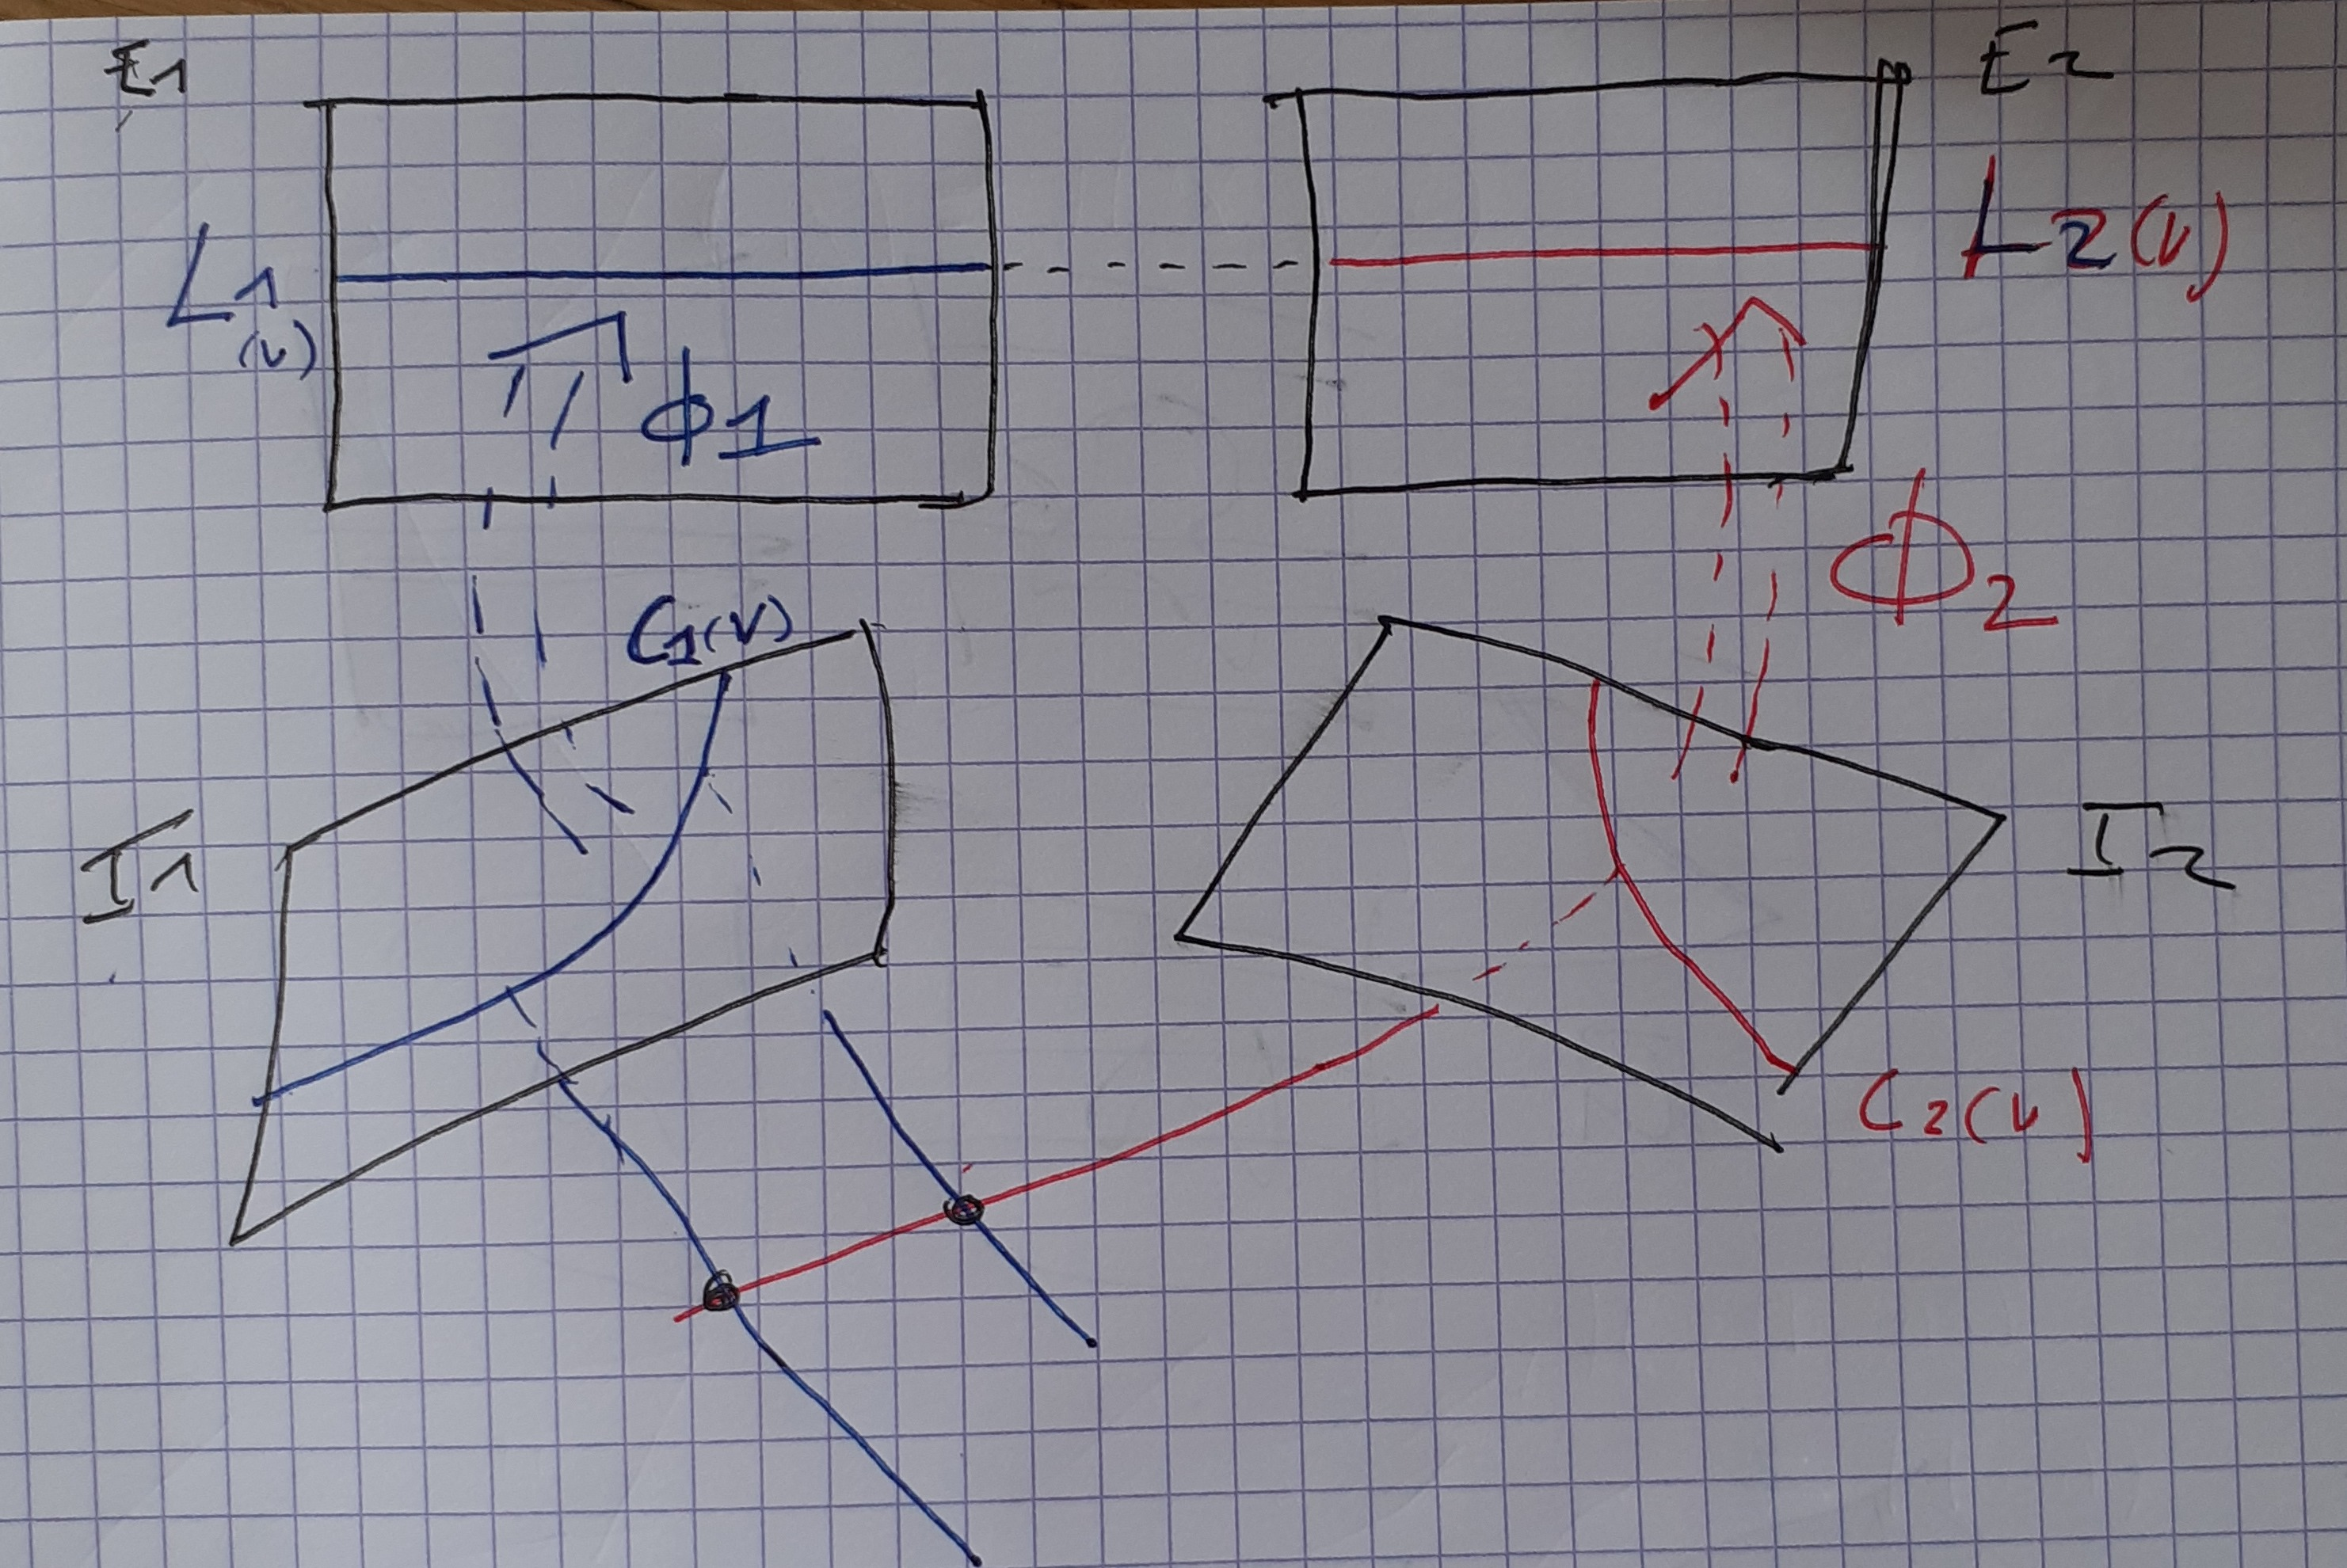
\includegraphics[width=15cm]{FIGS/Epip.jpg} 
 \\ \hline \hline
\end{tabular}
\caption{Illustration of epipolar geometry.}
\label{FigDefEpip}
\end{figure}


\noindent The matching of epipolar images is simplified because we know that the lines in two images are globally homologous. 
\er{The space of the image rectified to epipolar geometry is denoted by $E$ (see Figure~\ref{FigDefEpip})}


\begin{notation}[Epipolar line and curve.]
We note $\LineK(v)$   the epipolar  line of $E_k$ defined by $v_k=v$. We also note $\CurveK(v)$ the epipolar
curve of $I_k$ defined by $\CurveK(v) = \phi_k^{-1}(\LineK(v))$
\end{notation}
%
\noindent We can see that when epipolar geometry exists, the two curves $\CurveO(v)$ and $\CurveT(v)$ are globally homologous:

\begin{equation}
     \CurveO(v) = \PiOT{C_2(v)}   ;  \CurveT(v) = \PiTO{C_1(v)} \label{Eq:CurvHom}
\end{equation}


%---------------------------------------------

\subsection{Existence of epipolar geometry}

We now discuss the existence of {epipolar geometry}. As you will see, epipolar geometry generally does not exist, and when it does, it is not
unique. It is well known that:

\begin{itemize}
    \item for any image pair following the central projection there exists  an epipolar geometry;

    \item  not all image pairs can be resampled to epipolar geometry; for example, a cylindrical projection, applicable to many push-broom satellites, generally does not allow for epipolar resampling.

\end{itemize}
We explain now why epipolar geometry does not exist for any $\pi_1,\pi_2$ and is rather an exception. Let's define the surface $\Sv^k$ of $\RR^3$ by :

\begin{equation}
   \Sv^k = \pi_k^{-1}(\CurveK(v)).  \label{Svk}
\end{equation}
Following the definition of the \er{epipolar geometry}, it can be seen that $\Sv^1$ and $\Sv^2$ are the same surface $\Sv$:

\begin{equation}
   \Sv^1 = \Sv^2 = \Sv,
\end{equation}
which is a direct consequence of definitions. For any $P\in\Sv^1$, set  $e_1=\phi_1(\pi_1(P))=(u_1,v)$
and $e_2=\phi_2(\pi_2(P))=(u_2,v_2)$, we have $\pi_1(P) \HComp \pi_2(P)$ because they are projections
of the same point. Then, $v_2=v$ according to Definition~\ref{EqEpiEgalY} and $P \in \Sv^2$. Furthermore, the $\Sv$ defines a foliation of $\RR^3$, and it can be seen that:

\begin{equation}
   \forall v \forall P \in \Sv :  \BundO(P) \subset \Sv , \BundT \subset \Sv, \label{ClothureBundle}
\end{equation}
which is again a direct consequence of definitions, if $P \in \Sv$ then $\pi_k^{-1}(P) \in \CurveK(v)$
(see Equation~\ref{Svk}), then $\pi_k^{-1}(\pi_k(P)) = \BundK(P) \subset \Sv$.


But the existence of a stable foliation for the two bundles sets, as expressed in Equation~\ref{ClothureBundle},
cannot  be satisfied in general. It is  illustrated 
by Figure~\ref{FigClothPath} and explained in the following.  Let $\pi_1,\pi_2$ be any two  projections and suppose
there exists  a folliation satisfying the Equation~\ref{ClothureBundle}. Then, 

\begin{itemize}
   \item  let $P$ be any point of ground space, and $\Sv$ be the surface such that $P \in \Sv$;
   \item  let $P_1 \neq P$ be a point on $\BundO(P)$, $P_1 \in \Sv$, then $\BundT(P_1) \subset \Sv$;
   \item  let $P_2 \neq P$ be a point on $\BundT(P)$, $P_2 \in S_v$, then $\BundO(P_2) \subset \Sv$;
   \item  as $\BundT(P_1)$ and $\BundO(P_1)$ are included in the same surface $\Sv$ they
            must intersect somewhere in a point $Q$.
\end{itemize}
The above is a contradiction because, in the general case, there is no reason that for any two sets
of bundles the condition $\BundT(P_1) \cap \BundO(P_2) \neq \emptyset $ is satisfied
(see Figure~\ref{FigClothPath} on the right).

\begin{figure}
\centering
\begin{tabular}{||c|c||}
 \hline \hline
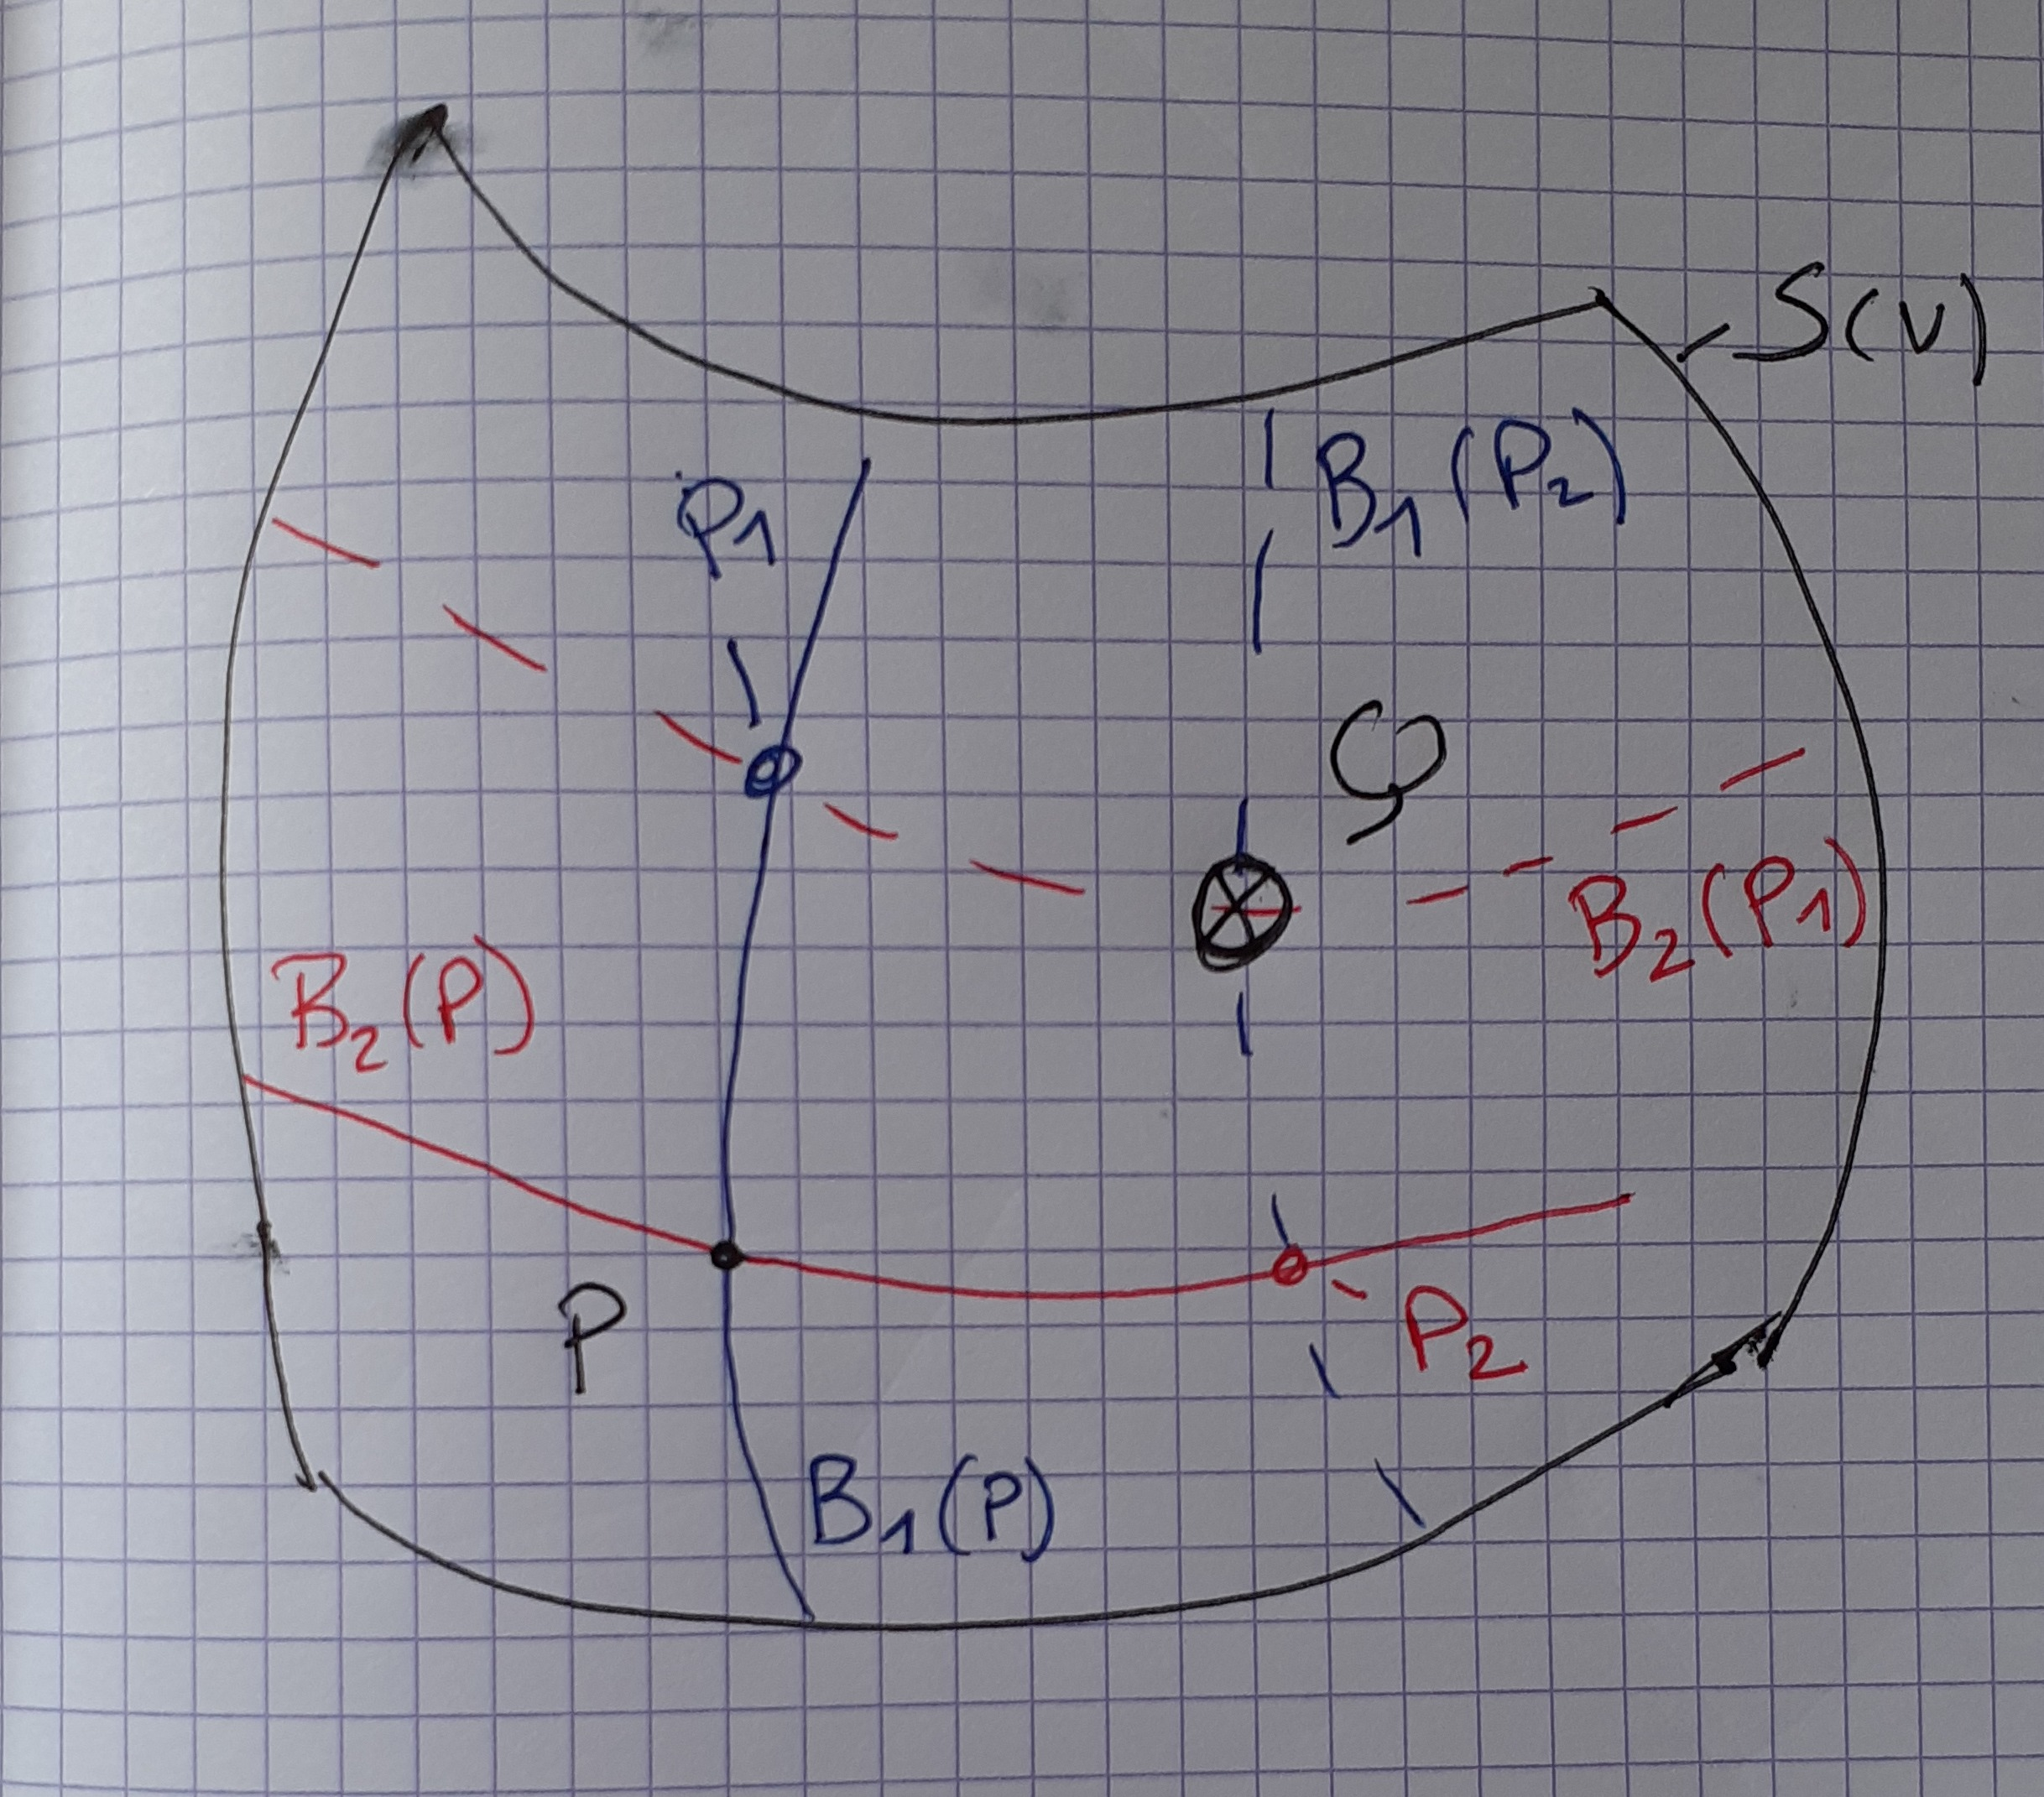
\includegraphics[width=8cm]{FIGS/ClothPathEpip.jpg} &
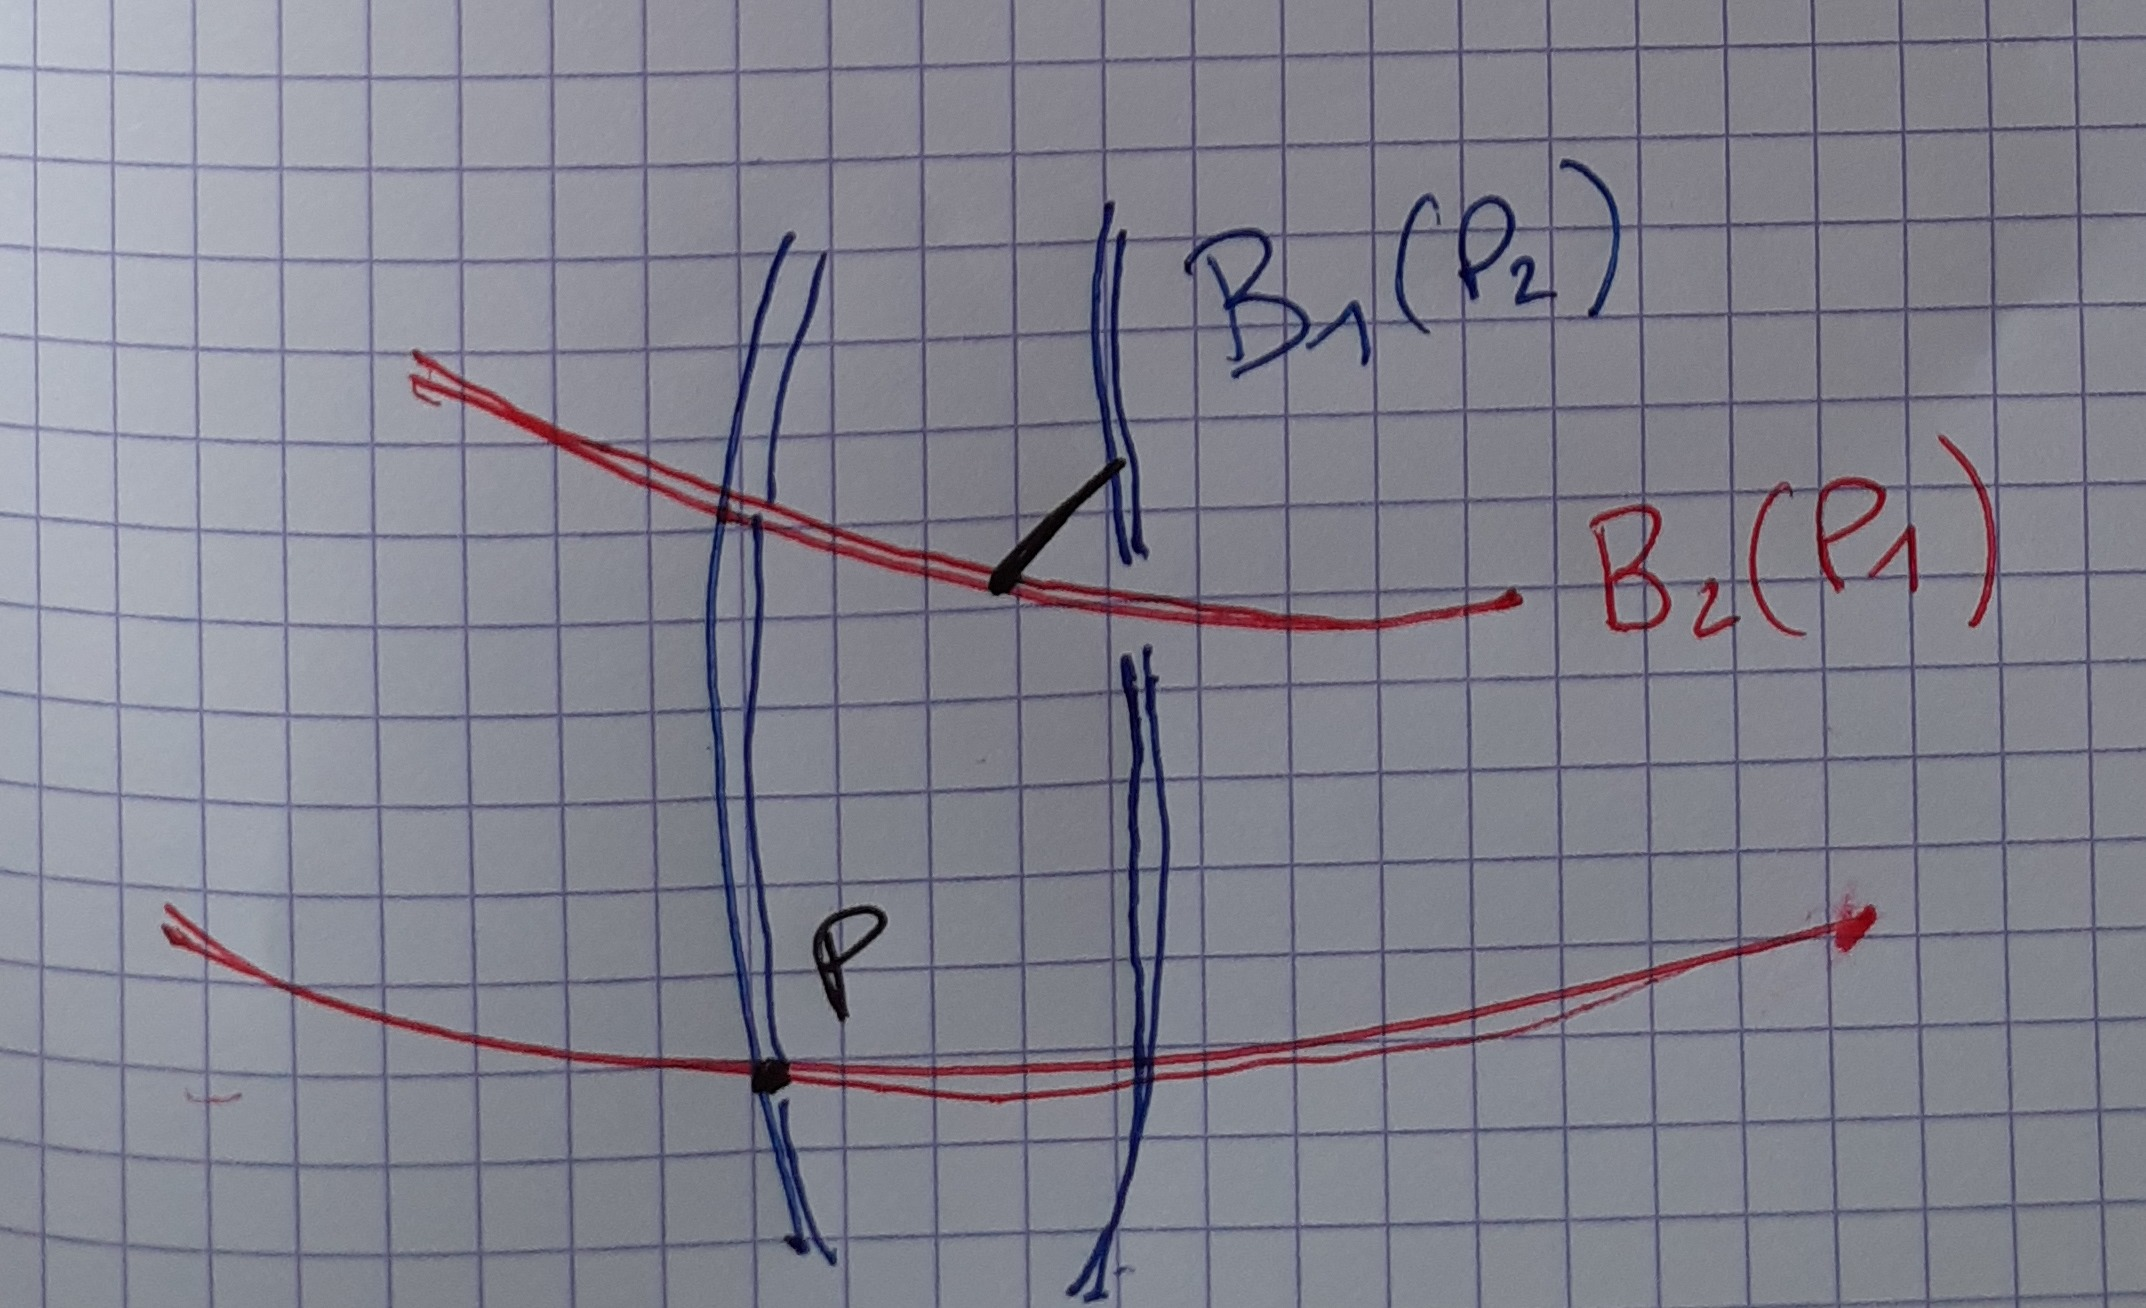
\includegraphics[width=8cm]{FIGS/ClothPathNonEpip.jpg} 
 \\ \hline \hline
\end{tabular}
\caption{Clothure of path . Left : epipolar case, the bundle are on the same level of a foliation and intersect.
Right : generic case, paht don't intersect, no epipolar can exist}
\label{FigClothPath}
\end{figure}

%---------------------------------------------


\subsection{A local caracterization of epipolar existence}

In this section we compute a local formula (i.e. a differential equation) that gives the conditions for
existence of an epipolar geometry. This section is rather theoriticall and
can be omitted for user interested mainly by practicall application.

\begin{figure}
\centering
\begin{tabular}{||c||}
 \hline \hline
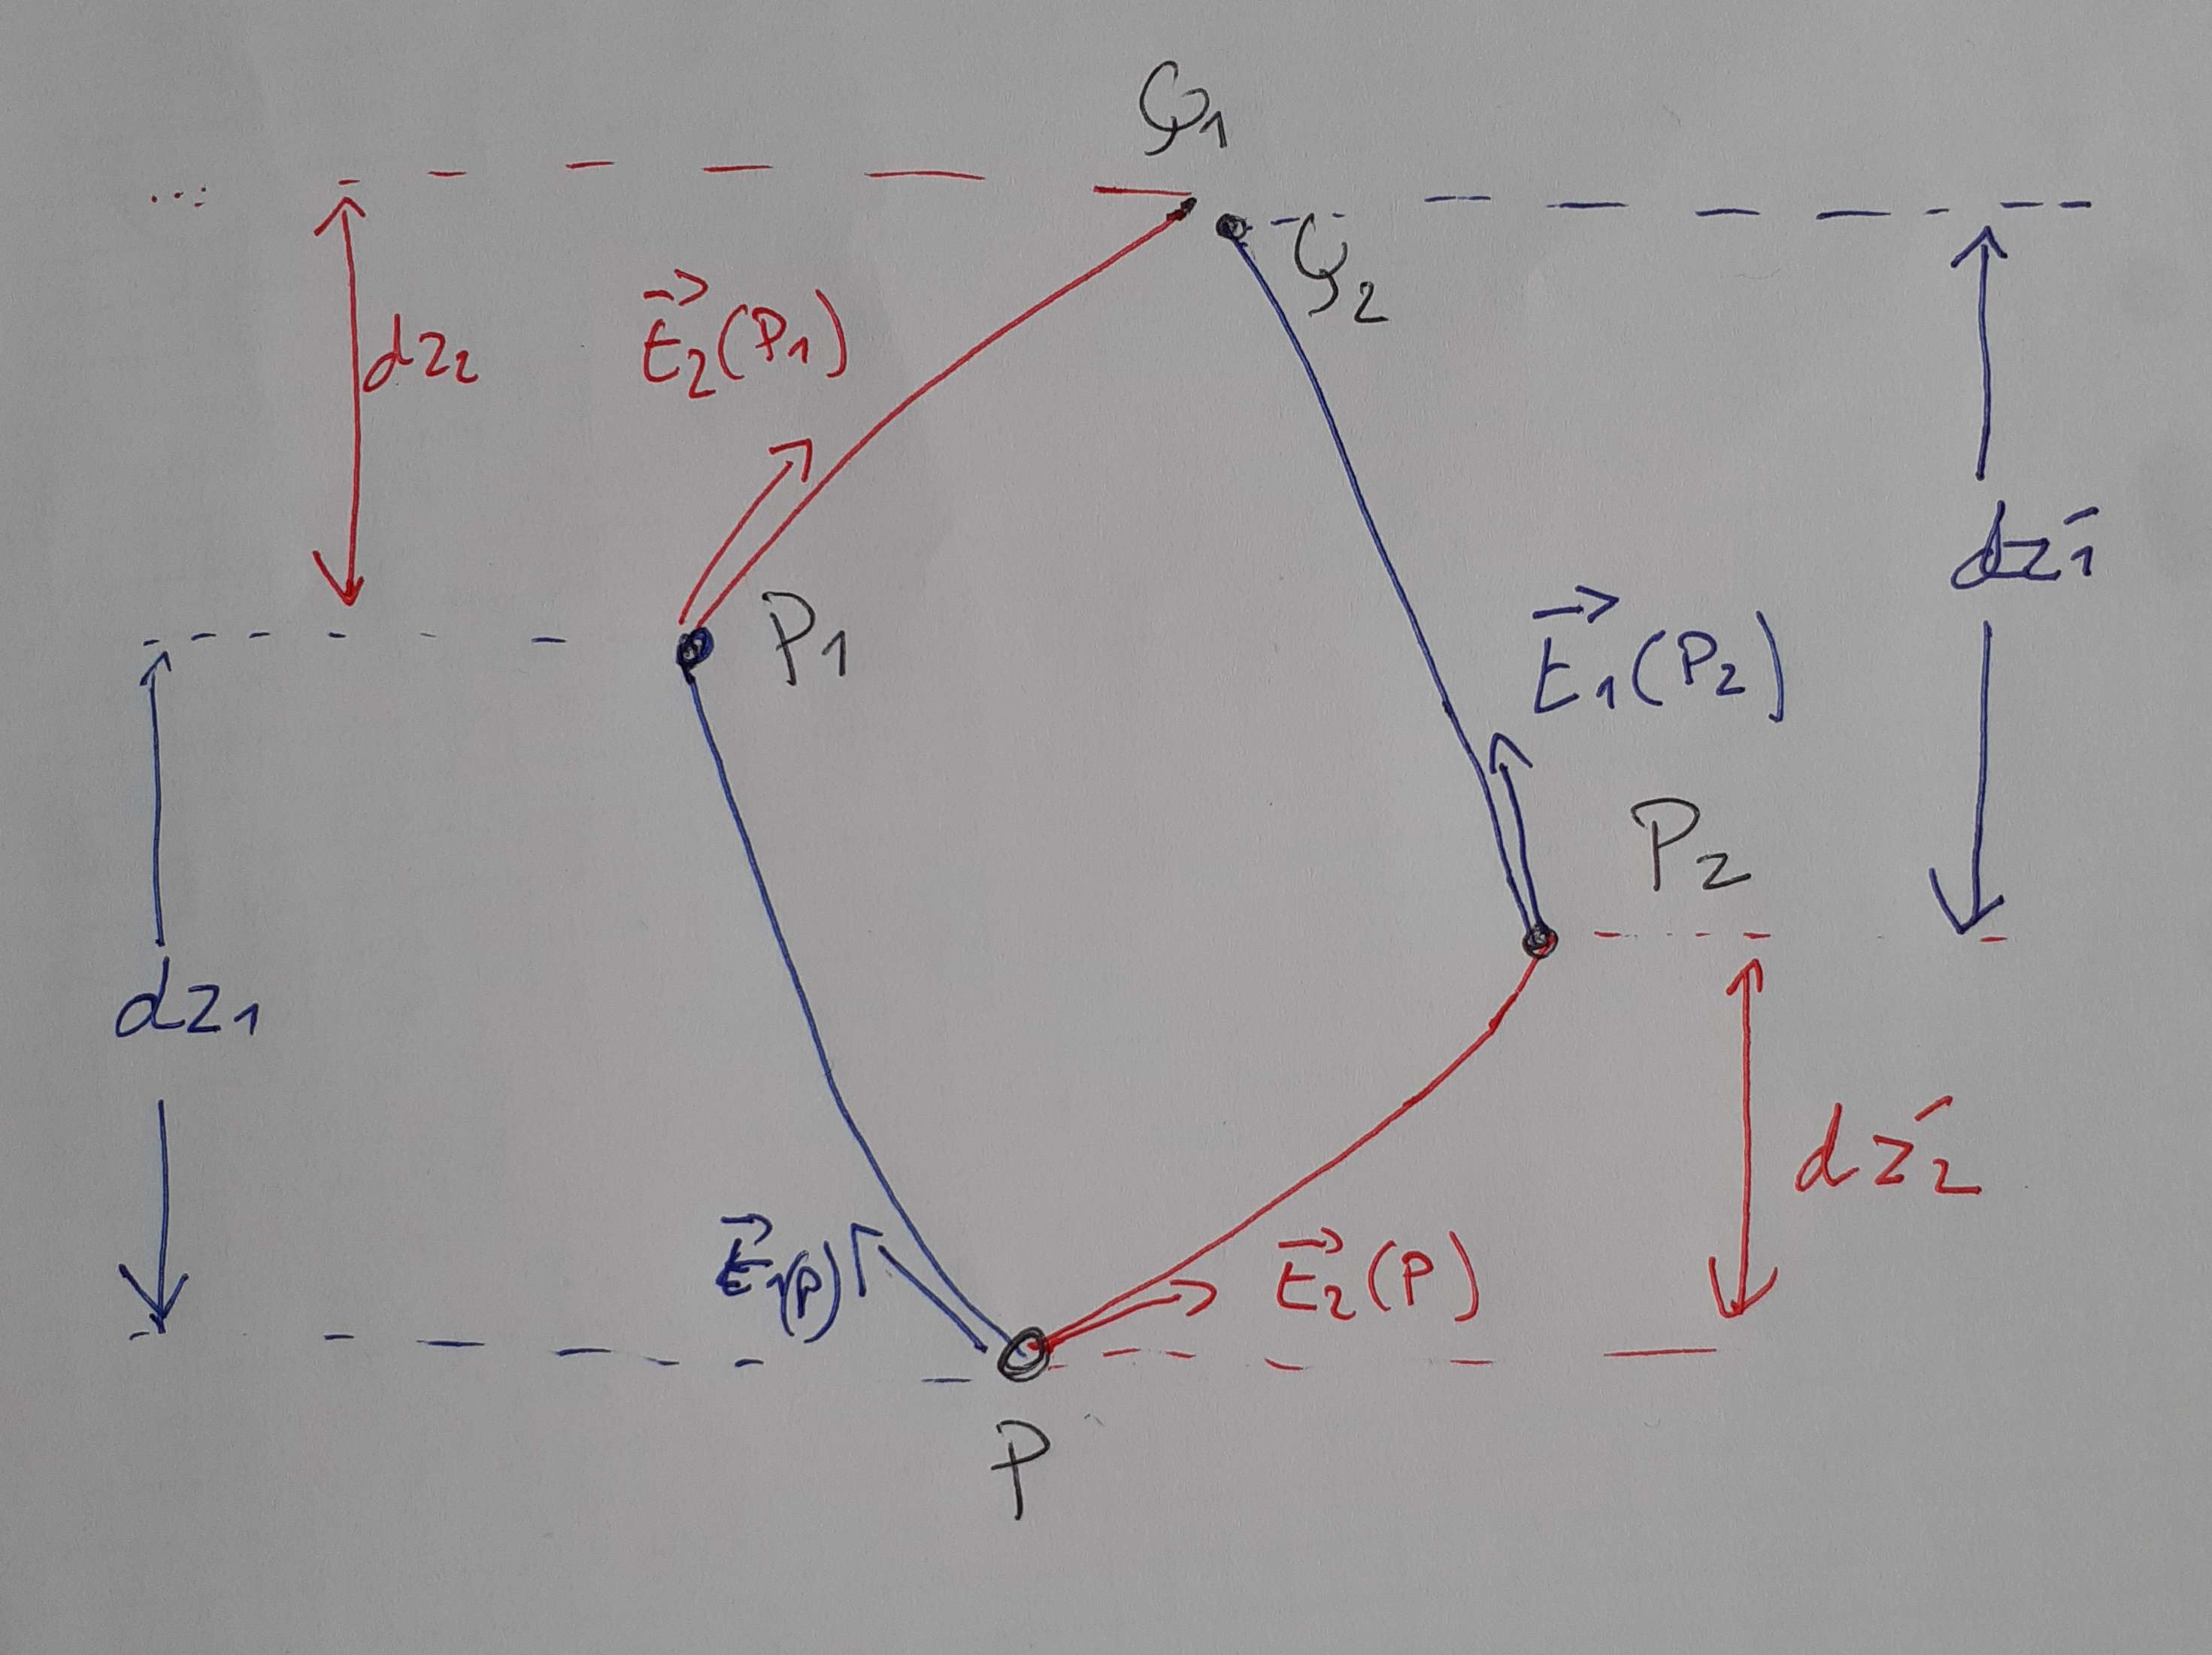
\includegraphics[width=10cm]{FIGS/EquadifEpip.jpg}
 \\ \hline \hline
\end{tabular}
\caption{Notation for local caracterization of epipolar existence}
\label{EqDifEpip}
\end{figure}

The idea is , as in section~\ref{ExistEpip}, is to make a  computation of pathes two way, $\BundO$ then $\BundT$ ,
and $\BundT$ then $\BundO$; then we express a taylor expansion of the intersection distance
between these two path.  We use the notation of figure~\ref{EqDifEpip} :

\begin{itemize}
   \item we make the sub-vertical assumption \footnote{when this assumption can be made,
          not we could use curvilinear abscisse};
   \item let $P$ be any point of $\RR^3$;
   \item consider a first path $(P,P_1,Q_1)$ following  $\BundO$ then $\BundT$ , making a
         progression $d_{z1}$ on $\BundO$ and  $d_{z2}$ on $\BundT$ ;
   \item consider a second path $(P,P_2,Q_2)$ following  $\BundT$ then $\BundO$ , making a
         progression $d_{z'2}$ on $\BundO$ and  $d_{z'1}$ on $\BundT$ ;
   \item we note $\overrightarrow{t_1(P)}=(x,y,1)$ the tangent to bundle  $\BundO$  in point $P$
         (and similarly $\overrightarrow{t_2}(P)$);
   \item when we will write  $\DerPart{F}{z_1}$ we will refer to the coordinate system $(i_1,j_1,z) = \PiVert_1^{-1}(x,y,z)$,
         idem for  $\DerPart{F}{z_2}$, and obviously as they are two different coordinate systems, we have in general
        $\DerPart{F}{z_1}  \neq \DerPart{F}{z_2}$;
\end{itemize}

Now, whatever may be the pair of 'small' values $(\delta_1,\delta_2)$,  we will compute the  pair of values
$(\delta'_1,\delta'_2)$ that minimize the distance $|Q_1,Q_2|$ and express the annulation of the
second degree taylor expansion of this distance (the first degree can always being annulated as we will see). 
Noting $\delta$ the max of all $\delta$, the degree $2$ Taylor expansion gives :

\begin{equation}
    P_1 =  P +  \delta_1 \TanO{(P)} + \frac{{\delta_1}^2}{2} \DerPart { \TanO{}}{z_1}(P)  + \Negl{\delta^3} \label{P1} 
\end{equation}
\begin{equation}
    Q_1 =  P_1 +  \delta_2 \TanT{(P_1)} + \frac{{\delta_2}^2}{2} \DerPart { \TanT{}}{z_2}(P_1) + \Negl{\delta^3} \label{Q1}
\end{equation}
\begin{equation}
     \TanT{(P_1)} = \TanT{(P)} +  \delta_1   \DerPart { \TanT{}}{z_1}(P) + \Negl{\delta^2} \label{TP1}
\end{equation}

Putting together equations~\ref{P1},~\ref{Q1},~\ref{TP1} we can make a taylor expansion of path
$P$ to $Q_1$ :

\begin{equation}
    Q_1 =    P +  \delta_1 \TanO{(P)} 
               +  \delta_2 \TanT{(P)} 
               + \frac{{\delta_1}^2}{2} \DerPart { \TanO{}}{z_1}(P) 
               + \frac{{\delta_2}^2}{2} \DerPart { \TanT{}}{z_2}(P) 
               +  \delta_1  \delta_2  \DerPart { \TanT{}}{z_1}(P)  
               + \Negl{\delta^3}
       \label{Q1ofP}
\end{equation}

And similarly for $P$ to $Q_2$ :

\begin{equation}
    Q_2 =    P +  \delta'_2 \TanT{(P)} 
               +  \delta'_1 \TanO{(P)} 
               + \frac{{\delta'_2}^2}{2} \DerPart { \TanT{}}{z_2}(P) 
               + \frac{{\delta'_1}^2}{2} \DerPart { \TanO{}}{z_1}(P) 
               +  \delta'_1  \delta'_2  \DerPart { \TanO{}}{z_2}(P)  
               + \Negl{\delta^3}
       \label{Q2ofP}
\end{equation}

The firts degree Taylor expansion of $Q_2-Q_1$ gives :

\begin{equation}
    Q_2 -Q_1 =   (\delta'_1 -\delta_1) \TanO{(P)} +  (\delta'_2 -\delta_2) \TanT{(P)}  + \Negl{\delta^2}
\end{equation}

To minimize $|Q_2 -Q_1|$, the first step is to annulate the degree $1$ terms of $ Q_2 -Q_1$ . We assume
that $\TanT{(P)}$ and $\TanO{(P)}$  are independant vectors~\footnote{elsewhere, it would be a 
degenerate case of stereovision} and we must then make of $\delta'_2 -\delta_2$ and $\delta'_1 -\delta_1$
term of degre $2$ :

\begin{equation}
   \Delta_1 =   \delta'_1 -\delta_1 = \Negl{\delta^2}  \; ; \; \Delta_2 =   \delta'_2 -\delta_2 = \Negl{\delta^2}
   \label{Delta}
\end{equation}

To develop $ Q_2 -Q_1$ we can use the following identities  that are direct consquences of~\ref{Delta} :

\begin{equation}
   \delta_1  \delta_2 -  \delta'_1  \delta'_2  = \Negl{\delta^3} \;;\;
   {\delta_1}^2 - {\delta'_1}^2 =  \Negl{\delta^3} \;;\;
   {\delta_2}^2 - {\delta'_2}^2 =  \Negl{\delta^3} 
   \label{NeglDelta}
\end{equation}

Subtracting \ref{Q1ofP} to \ref{Q2ofP}, and using~\ref{NeglDelta},we can write :

\begin{equation}
    Q_2 -Q_1 =   \Delta_1 \TanO{(P)} +   \Delta_2 \TanT{(P)}  
               + \delta_1  \delta_2(\DerPart { \TanT{}}{z_1}(P)  -\DerPart { \TanO{}}{z_2}(P) )
               + \Negl{\delta^3}
\end{equation}


We now traduce the intersection of path by annulating the degree $2$ Taylor expansion of $Q_2 -Q_1$.
We have  $3$ vector, and their weighted sum can be null, iff they are colinear.

\begin{theorem}[Existence of epipolar]
The epipolar exist iff the following determinant is null :

\begin{equation}
\left[ \begin{array}{c|c|c}
\TanO{} & \TanT{}  & \DerPart { \TanT{}}{z_1}  -\DerPart { \TanO{}}{z_2}  
\end{array} \right]  
=0
\end{equation}

\end{theorem}

\begin{remark}[Epipolar equation with central perspective camera]
As an illustration in an easy case, we can see that this condition is trivially 
satisfied for a pair of central perspective cameras as we have the annulation of both terms as shown
in equation~\ref{EqEpipConik}. This is because for a given point $P$,
for any point $P_1$ on $\BundO(P)$, $\TanT{P_1}$ belongs to the epipolar
plane $\mathcal{P}$ , we have $\TanT{P_1} \in \mathcal{P}$, so $\DerPart { \TanT{}}{z_1} \in \mathcal{P}$,
and as we have also $\TanO{(P)} \in  \mathcal{P}, \TanT{(P)} \in  \mathcal{P}$, the collineratity
between $\TanO{(P)}$ , $\TanT{(P)}$ and $\DerPart { \TanT{}}{z_1}(P)$ is proved.

\begin{equation}
\left[ \begin{array}{c|c|c}
\TanO{} & \TanT{}  & \DerPart { \TanT{}}{z_1}  
\end{array} \right]  
=\left[ \begin{array}{c|c|c}
\TanO{} & \TanT{}  & \DerPart { \TanO{}}{z_2}  
\end{array} \right]  
=0
\label{EqEpipConik}
\end{equation}
\end{remark}


%---------------------------------------------


\subsection{Ambiguity of epipolar geometry}

When the epipolar geometry exists, the epipolar resampling is not unique. To demonstrate that our rectification method handles this ambiguity rigorously, we first describe it formally. Let $\phi_1,\phi_2$ and  $\phi'_1,\phi'_2$ be two   epipolar resamplings.
For any pair of lines $\LineK(v)$ in $E_k$, there are corresponding 
homologous curves $\CurveO(v),\CurveT(v)$  in images 
$I_1,I_2$ (see Equation~\ref{Eq:CurvHom}). Following the depiction in Figure~\ref{FigAmbigEpip}, if $\phi'_k(\CurveK(v)))$
are  lines $\LineK(v')$ in $E_k$, one can observe that $\phi'_1 \phi_1^{-1}$  and $\phi'_2 \phi_2^{-1}$ are diffeomorphisms transforming lines in lines, and they globally \er{operate the same transformation on lines.}
And \textit{vice versa}, let  $\phi_1,\phi_2$ be an epipolar resampling and let $\Lambda_1,\Lambda_2$ 
be diffeomorphisms  that are stable for lines and make globally the same transformation on lines. We can thus note that $\Lambda_1 \circ \phi_1$ and  $\Lambda_2 \circ \phi_2$ are also an epipolar resampling.


Having devised the exact ambiguity, we can now define two constraints to impose a unique epipolar resampling: 
\begin{enumerate}
\item Constraint on uniqueness of the deformation
inside each line of each \er{function}. For instance, one can impose that the colums remain constant (i.e.
the deformation is made only on  $y$), as given in Equations~\ref{Ambig:PhiO}
and~\ref{Ambig:PhiT};
\item Constraint on the global deformation of lines\footnote{i.e. where each line
is transformed globally to another line}. For instance, by fixing the transformation of one image, as given Equation~\ref{FigAmbigEpip}.
\end{enumerate}
 

\begin{figure}
\centering
\begin{tabular}{||c||}
 \hline \hline
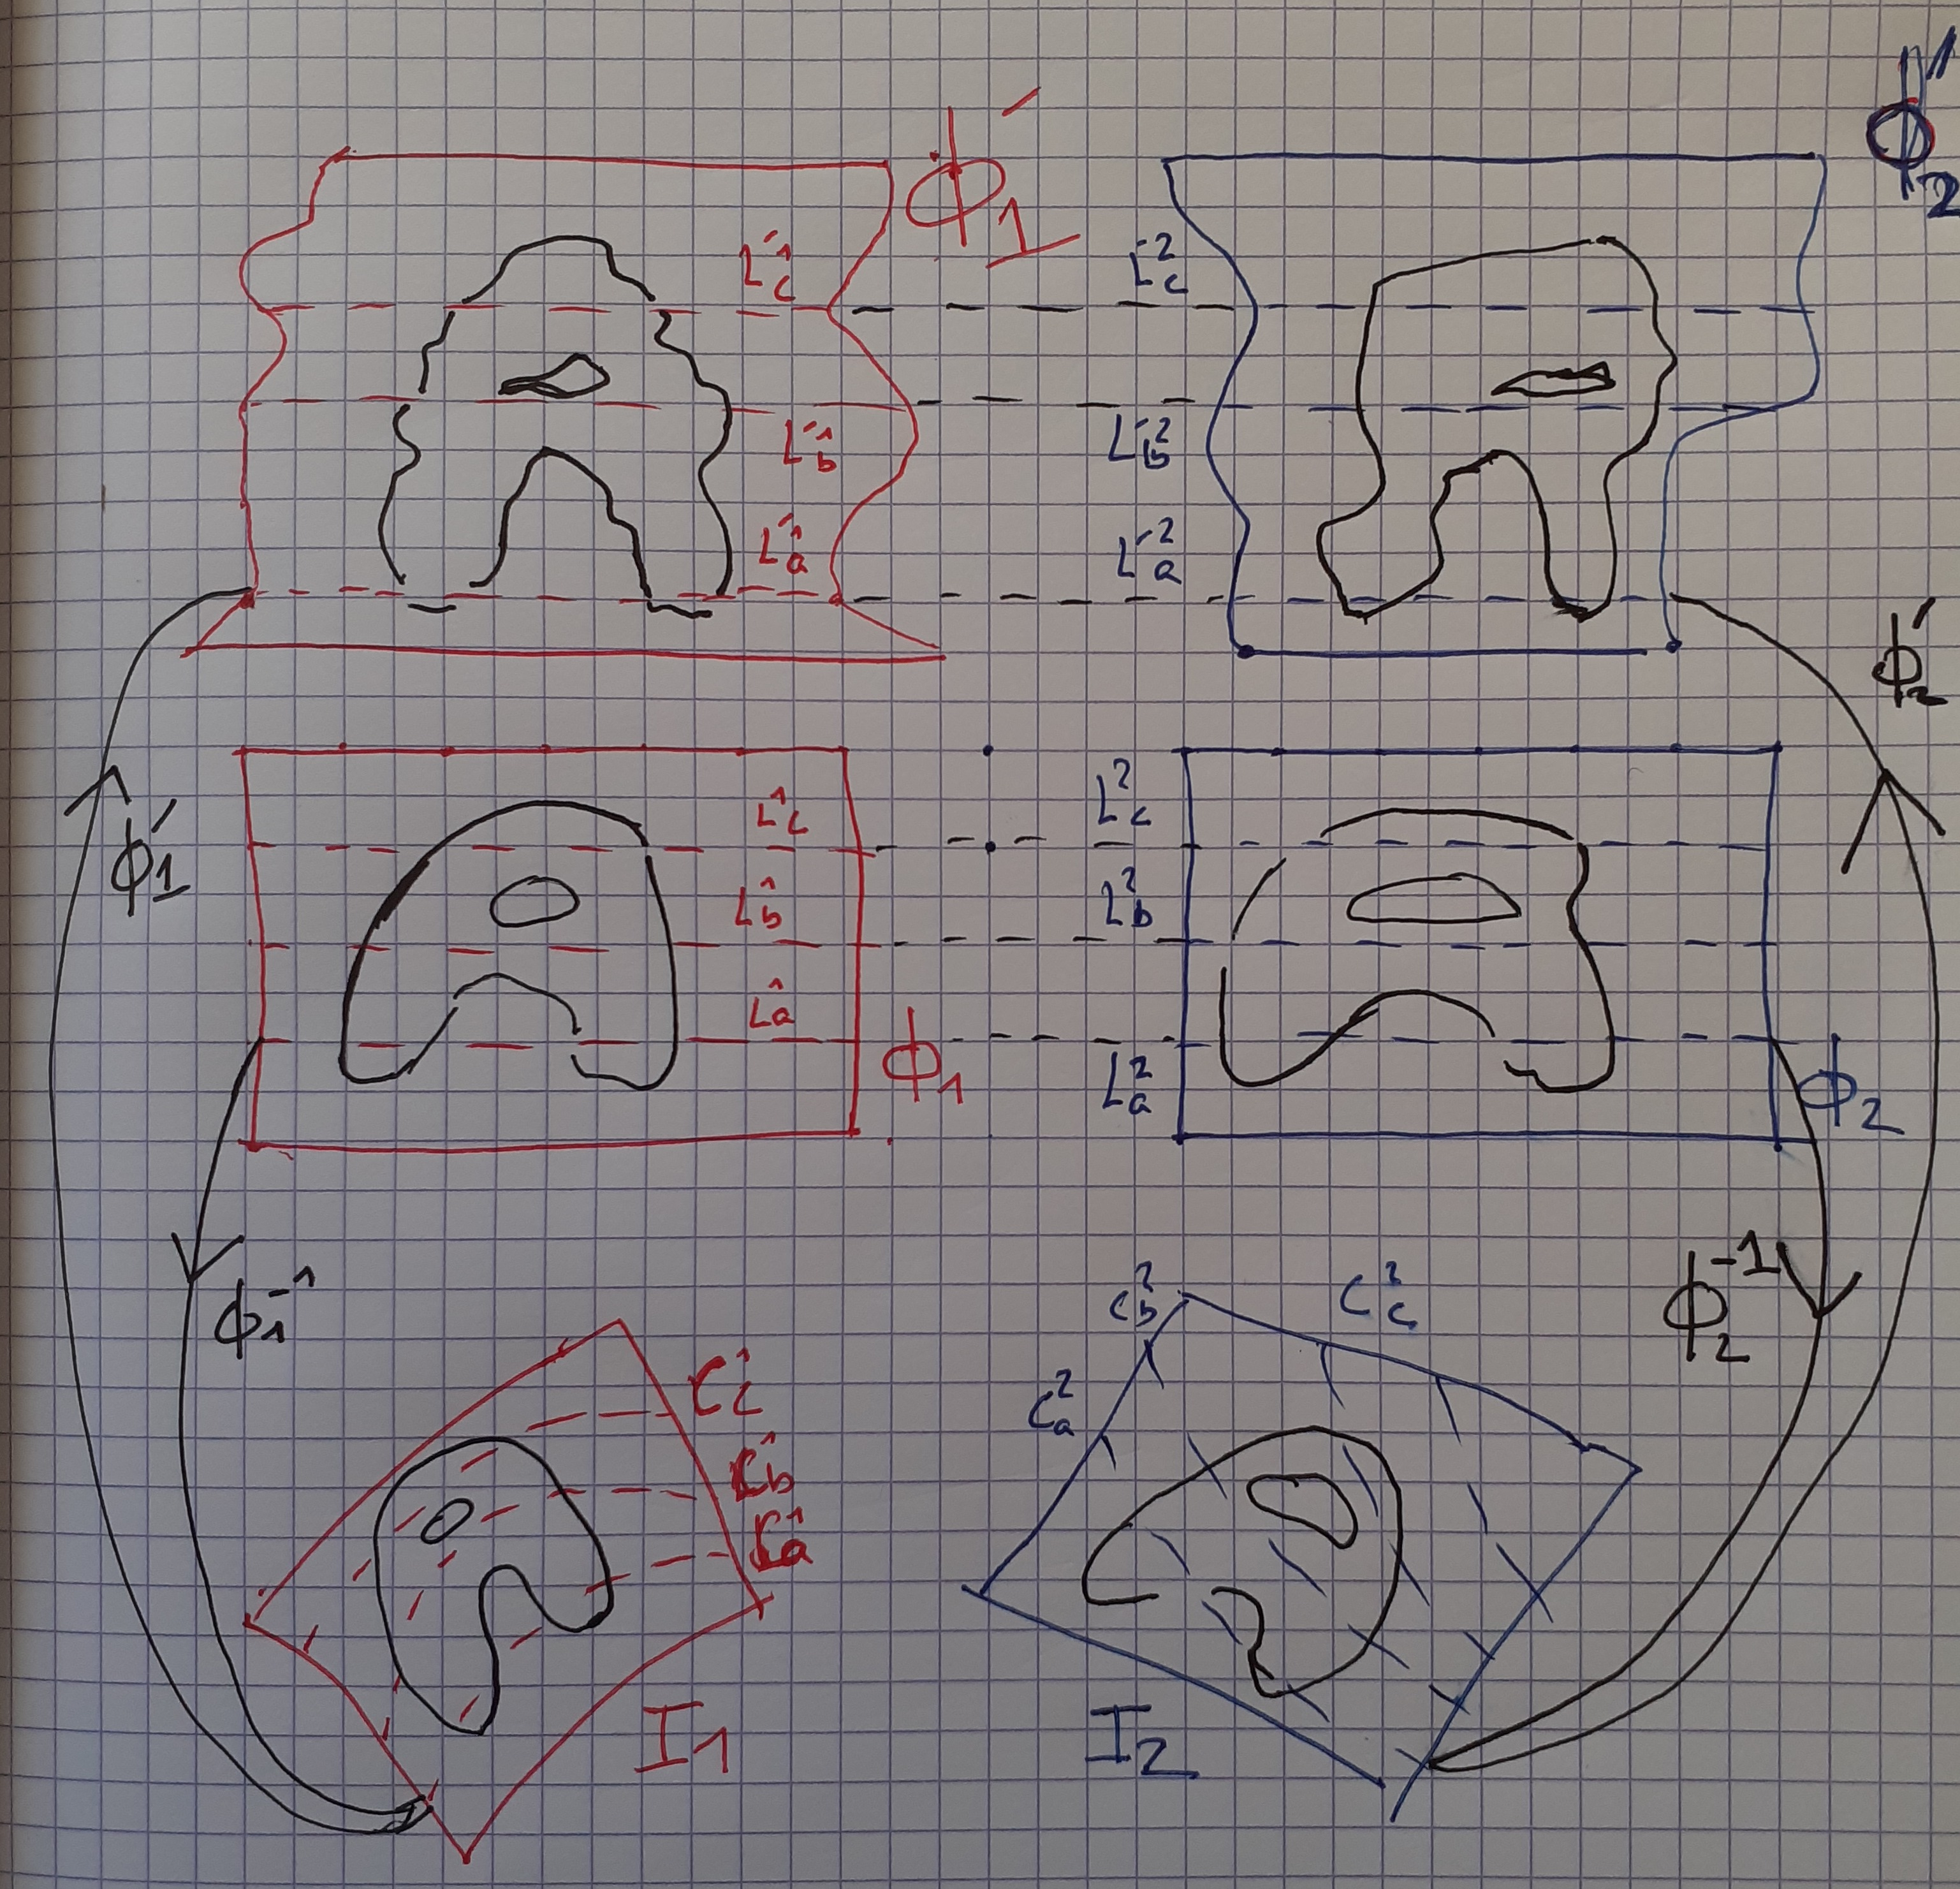
\includegraphics[width=10cm]{FIGS/AmbigEpip.jpg}
 \\ \hline \hline
\end{tabular}
\caption{Ambiguity : two possible epipolar resampling}
\label{FigAmbigEpip}
\end{figure}




\begin{theorem}[Unique epipolar constraint]

If epipolar geometry exists, there exist a unique epipolar resampling $\phi_1,\phi_2$ satisfying the $3$ following constraints:

\begin{equation}
    \phi_1(x,y) = (x,y') \label{Ambig:PhiO}
\end{equation}
\begin{equation}
    \phi_2(x,y) = (x,y') \label{Ambig:PhiT}
\end{equation}
\begin{equation}
    \phi_1(0,y) = (0,y) \label{Ambig:Line}
\end{equation}
\label{Theo:Fix:Ambig}

\end{theorem}



%---------------------------------------------
%---------------------------------------------
%---------------------------------------------

\section{Proposed method for epipolar ressampling}


\subsection{Hypothesis and layout}

\subsubsection{Principles}
The principle of the methods is to use \emph{H-Compatible}  points $p_1,p_2$ to calculate a
pair of function $\phi_1,\phi_2$ that complain with the epipolar constraint :
\emph{"$\phi_1(p_1)$ and $\phi_2(p_2)$ are on the same line"}. As these epipolar function
are not unique, in application of theorem~\ref{Theo:Fix:Ambig} we  parametrize $\phi_k$ according to following equation :


\begin{equation}
    \phi_k(i,j) = (i,V_k(i,j))  \; \; ; \; \;
    V_k : \RR^2 \rightarrow \RR  
  \label{EpipVParam}
\end{equation}

This parametrization handle  equation~\ref{Ambig:PhiO} and~\ref{Ambig:PhiT}; 
we will see later \footnote{see equation~\ref{CstrV1:0} and ~\ref{CstrV1:1} in section~\ref{ChoicePolyn}}
how we handle equation \ref{Ambig:Line}.
For  computing $V_1,V_2$ , for any pair of \emph{H-Compatible} points we add the observation
of equation~\ref{EqV1V2} that constraint $V_1$ and $V_2$ :


\begin{equation}
    V_1(p_1) = V_2(p_2) \label{EqV1V2}
\end{equation}

\subsubsection{Hypothesis}


The method take as input two geometric models of the camera $\pi_1$ and $\pi_2$.
These models are regarded as "black box" satisfying the equation~\ref{Eq:Proj} and the method 
make no specific assumption on the physical model of the camera. In our own \CPP implementation,
the cameras are regarded as pure virtual classes offering interface to equation~\ref{Eq:Proj}.
In this paper, the examples processed by our method are RPC satellite models and frame camera (central perspective) but the
only restriction in on the "smoothness" of the projection function :

\begin{itemize}
    \item the fact that $\pi$ are   $\mathcal{C}^{\infty}$ function;
    \item the fact that the direction of epipolar curves have a limited interval of variation (say for example
          less than $\frac{\pi}{2}$).
\end{itemize}

\begin{figure}
\centering
\begin{tabular}{||c||}
 \hline \hline
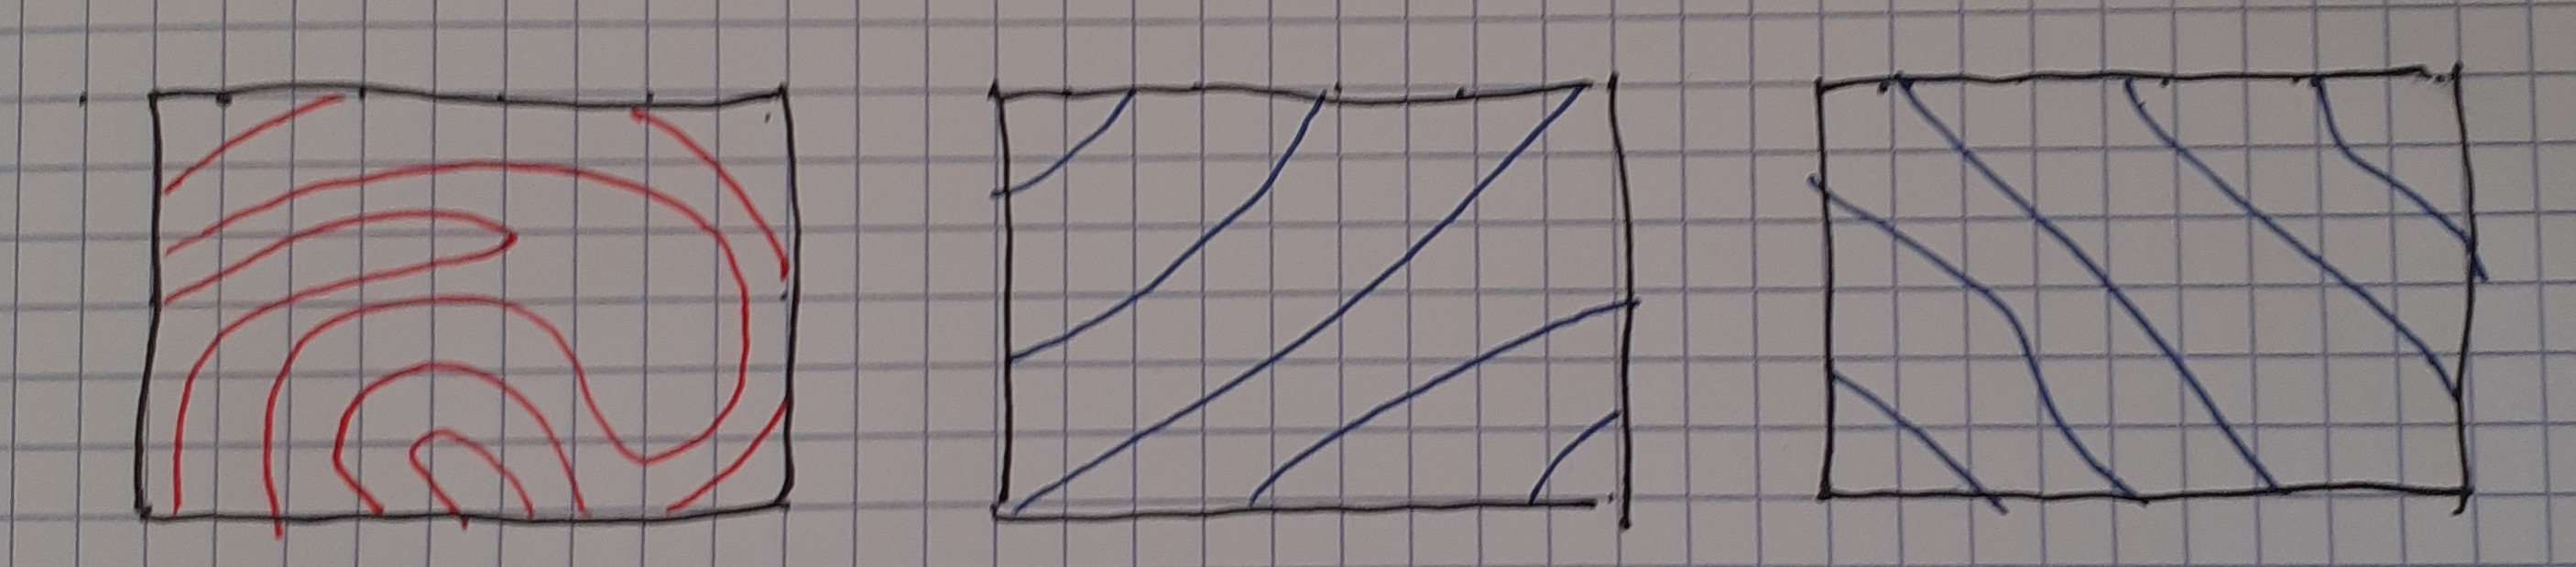
\includegraphics[width=10cm]{FIGS/BadGoodLines.jpg}
 \\ \hline \hline
\end{tabular}
\caption{Left : a set of epipolar line not handled with our methods. Right : a perfectly acceptable pair  of epipolar line}
\label{BadGoodEpip}
\end{figure}

Figure~\ref{BadGoodEpip} illustrates the last constraint on epipolar curves. Left image present a set
of epipolar line that would not be handled by our methods.  Right image, represent a pair of epipolar line
that would be handled without problem because for each of them the direction of the line are included
in a restricted interval. 


\subsubsection{Center and global direction estimations}

The mehod estimate first the center $C_1,C_2$ of set of points $p_1$ and $p_2$, this is done by
a simple computation of average of coordinates.  Then all the computation are done in
a repaire originate in this center. 

This operation is usefull for the  application of constraint~\ref{Ambig:Line} so that is applied
at the center of the data.



The method then estimates for each image the average direction $\vec{D}_k$
of its epolar line, and a rotation $R_k$ is applied to the data so that the epipolar line become
globally horizontal using formula of equation~\ref{EqRot}.
The  epipolar deformation is computed on these rotated data.

\begin{equation}
    R_k(p) =  \frac{p-C_k}{\vec{D}_k}  \label{EqRot}
\end{equation}


This setting in a repair where epipolar lines are globaly horizontal, is
a consequence of equations~\ref{EpipVParam}, and is illustrated by figure~\ref{ReqOrient} :

\begin{itemize}
   \item left image of figure~\ref{ReqOrient} presents a case where epipolar curve are quasi vertical
         and for which an epipolar correction, without initial rotation,  
          according to equation~\ref{EpipVParam} would be impossible;
   \item middle image of figure~\ref{ReqOrient} presents a case where epipolar curve are oblique,
         in this case epipolar correction according to equation~\ref{EpipVParam} would be possible
         but would lead to important distorsion in the image, as can be seen on left image.
\end{itemize}




\begin{figure}
\centering
\begin{tabular}{||c||}
 \hline \hline
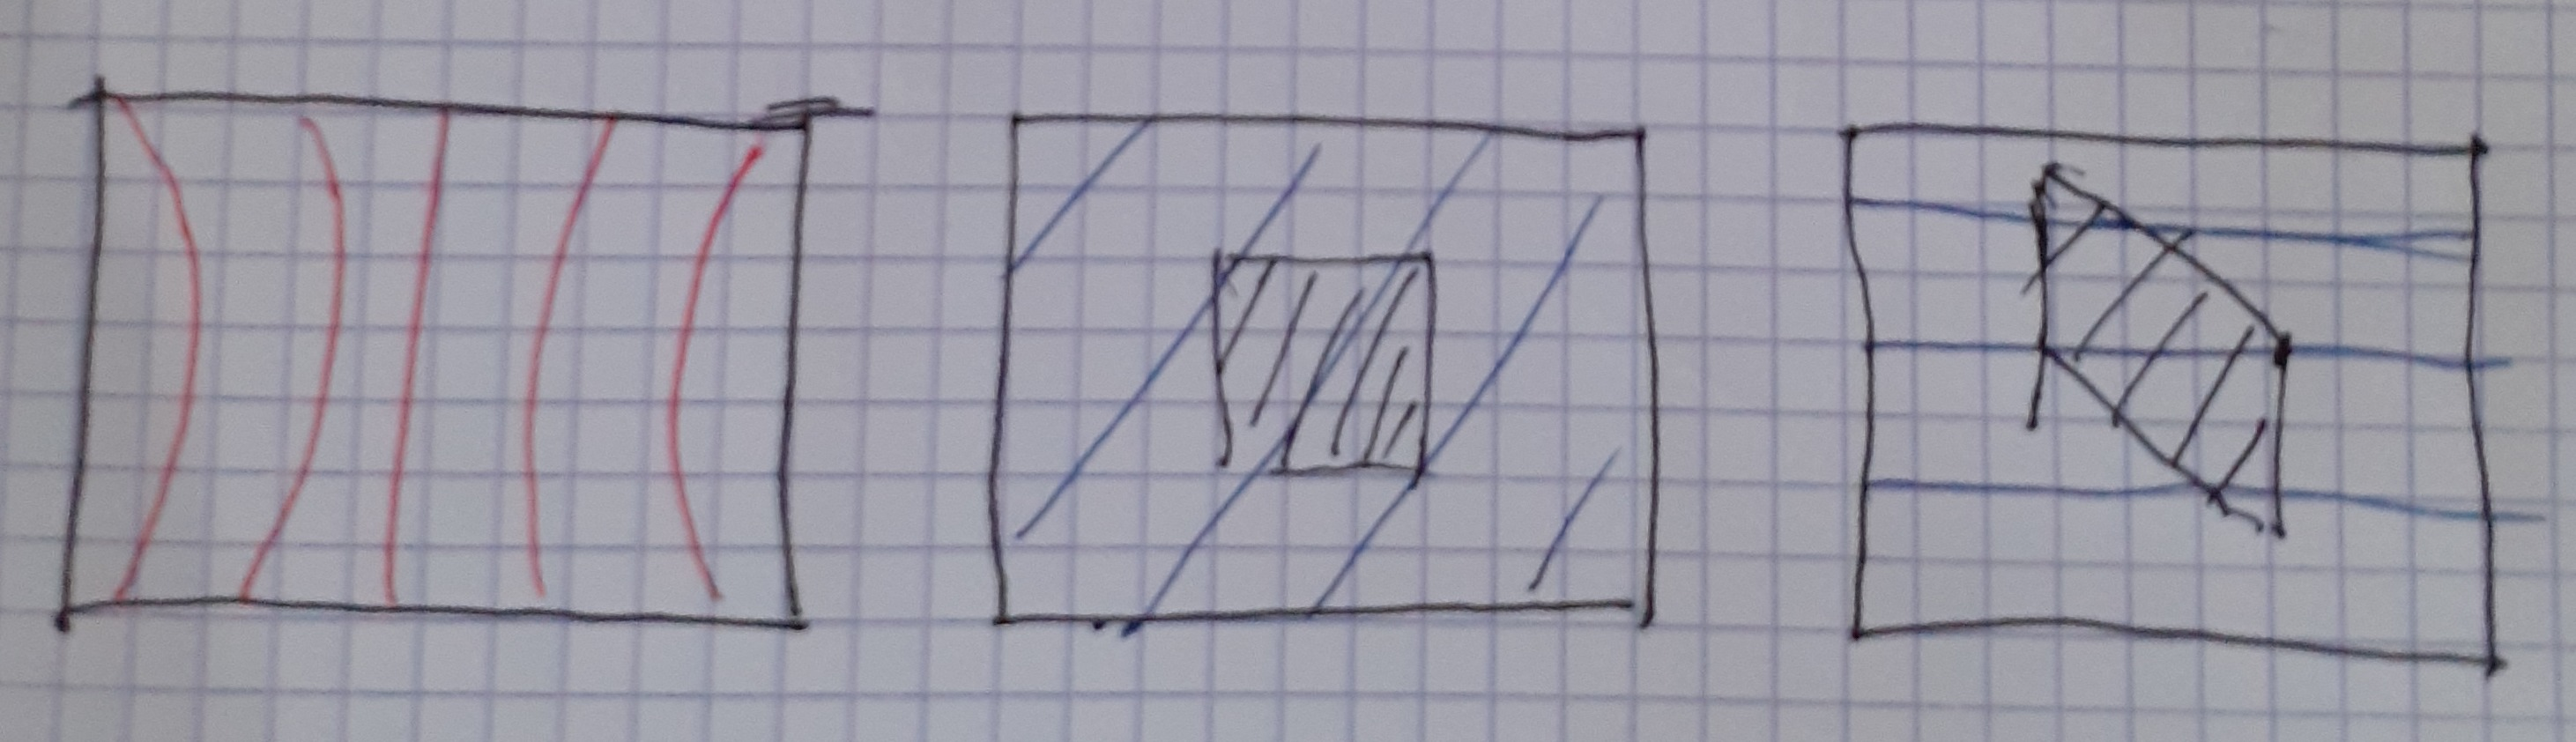
\includegraphics[width=10cm]{FIGS/EpipReqOrient.jpg}
 \\ \hline \hline
\end{tabular}
\caption{Left : quasi vertical epipolar curve, correction with equation~\ref{EpipVParam} is impossible. 
         Middle,Right  : oblique curve, epipolar rectification  with equation~\ref{EpipVParam} is possible
         but generate important distorsion}
\label{ReqOrient}
\end{figure}





\subsubsection{Layout}

The layout of the method we propose is then $3$ steps : (1) estimate the global 
direction of epipolar curve (2) estimate $F_1,F_2$ the local epipolar rectification
 in the repaire linked to these global direction (3)  estimate the final
epipolar rectification as a composition of $F_1,F_2$ and the rotation.
A more formalized description of the algorithm is given in bloc ~\ref{AlgoGlob}.


\begin{algorithm}
\caption{Epipolar($\pi_1$,$\pi_2$)}
\begin{algorithmic}
    \STATE {\emph{Layout of the algorithm for computing the epipolar rectification from camera models}}
    \STATE Use $\pi_1,\pi_2$ to estimate a set of \emph{H-Compatible} point $\mathcal{H} =\{(p_1,p_2)\}$ : 
    \STATE Estimate centers $C_1$ and $C_2$ ;
    \STATE Estimate global direction of epipolars $\vec{D}_1$ and $\vec{D}_2$ ,
    \STATE Estimate rotations $R_1,R_2$ according to formula~\ref{EqRot}
    \FORALL{$p_1,p_2 \in \mathcal{H}$}
              \STATE set : $q_1 = R_1(p_1)$,  $q_2 = R_2(p_2)$
              \STATE add equation : $V_1(q_1) = V_2(q_2)$
    \ENDFOR
    \STATE estimate by least square $V_1$ and $V_2$
    \STATE set $F_k(x,y)=(x,V_k(x,y))$  %, $F_2(x,y)=(x,V_2(x,y))$
    \STATE set $\phi_k =  F_k \circ  R_k $ % and $\phi_2=F_2 \circ R_2$
    \RETURN $(\phi_1,\phi_2)$
\end{algorithmic}
\label{AlgoGlob}
\end{algorithm}



\subsubsection{Why should it work ?}

Intuitively, it may be not obvious that the system of equation~\ref{EqV1V2} is well posed.
In fact, in the case where there would exist a functionnal relation between
$p_1$ and $p_2$ , as $p_1=F(p_2)$,  there would exist infinity of solution
for $(V_1,V_2)$ :   for any function $V: \RR^2 \rightarrow \RR $ we can generate a solution $(V\circ F, V)$ .

\begin{figure}
\centering
\begin{tabular}{||c||}
 \hline \hline
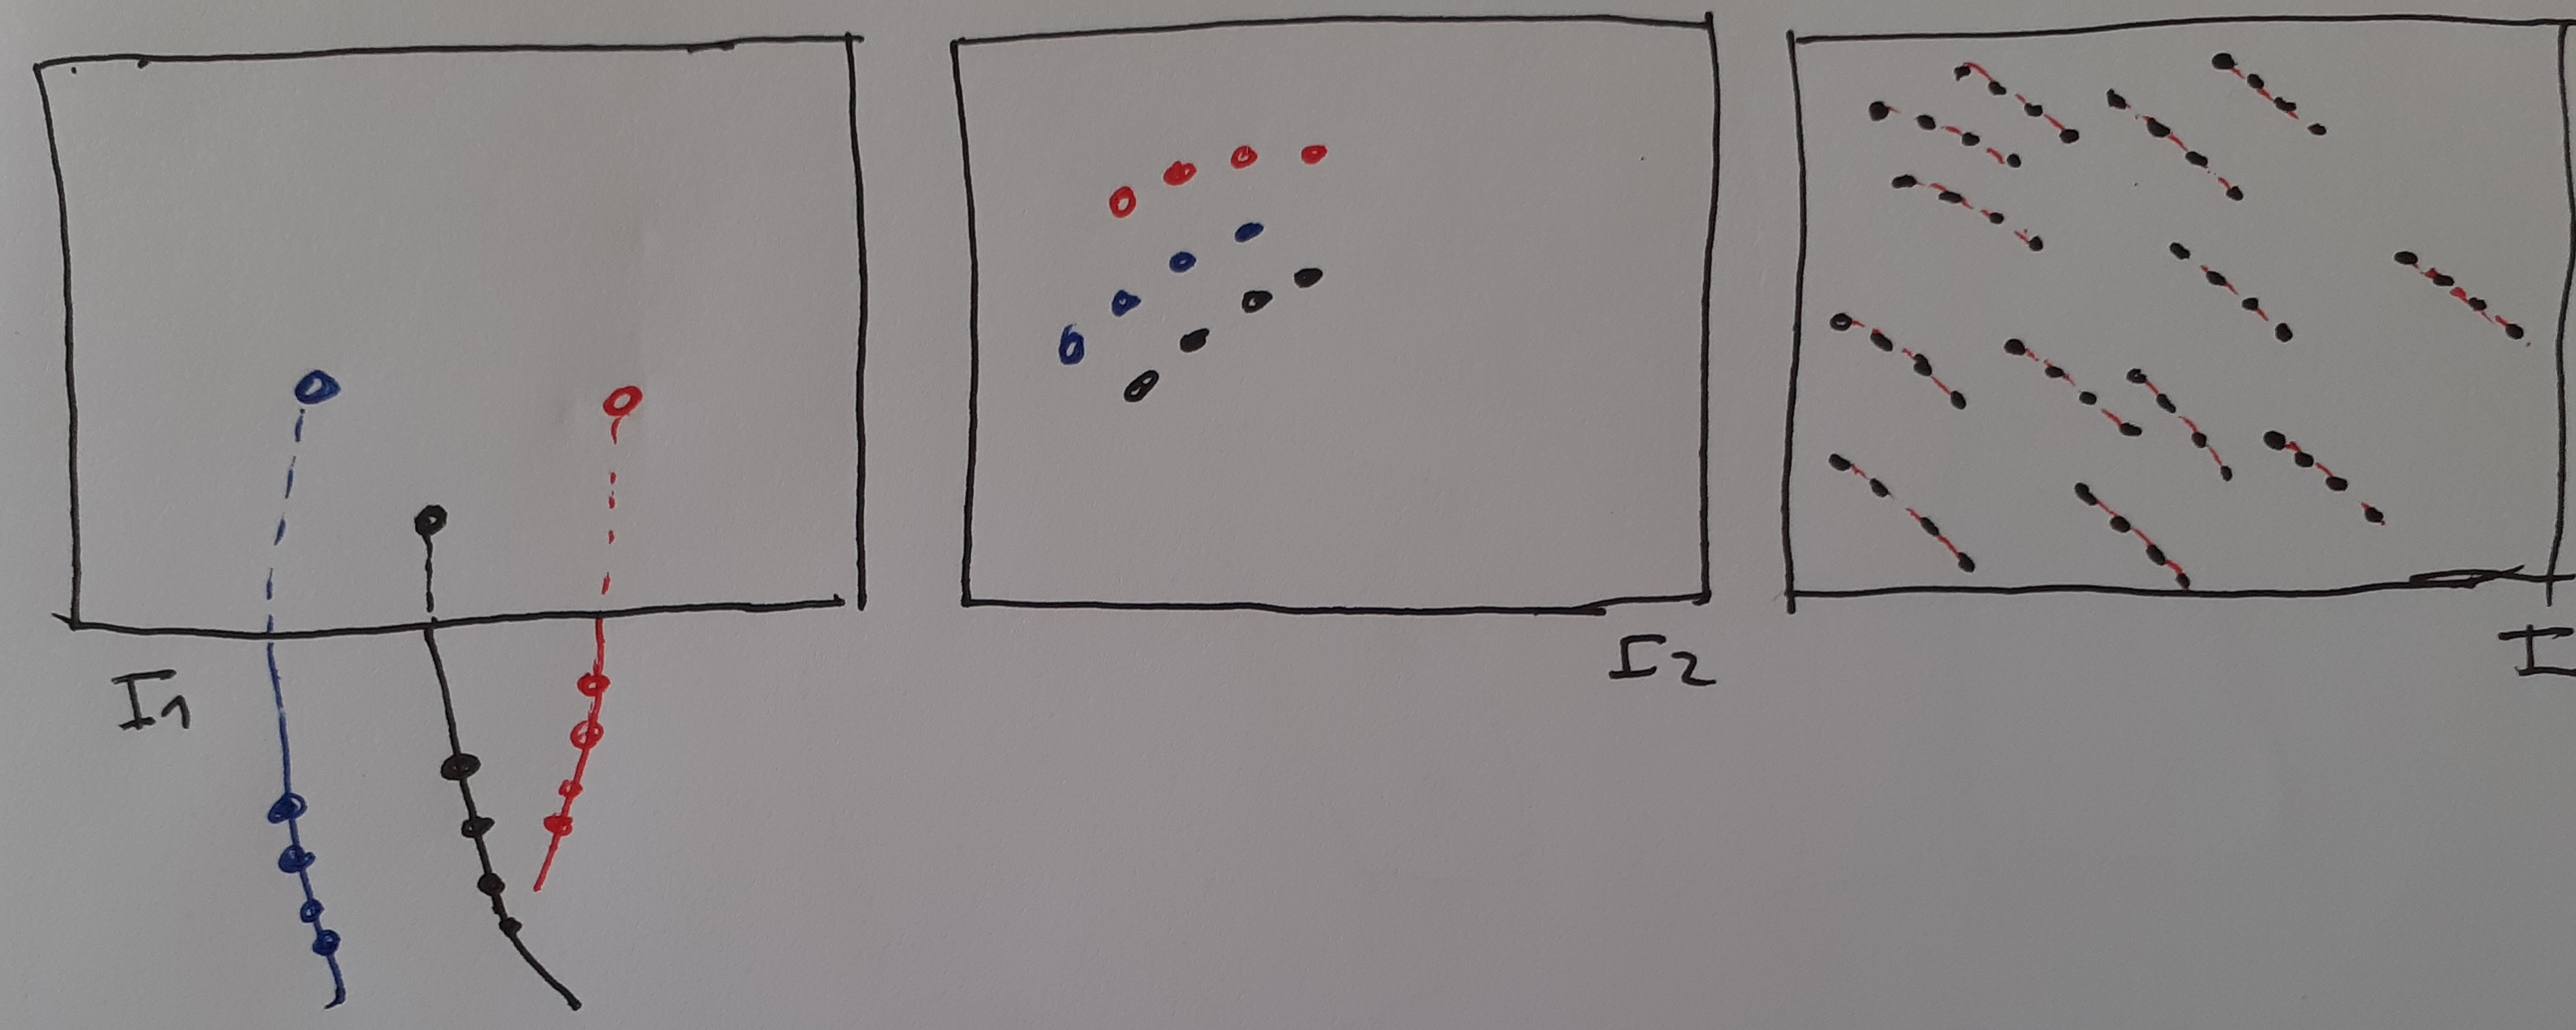
\includegraphics[width=10cm]{FIGS/NonFuncCorresp.jpg}
 \\ \hline \hline
\end{tabular}
\caption{Letft : for each $p_1$ we generate several $3d$ point on $B_1(p_1)$ . Middle :
         the multiple corresspondance in $I_2$ . Right : a dense network of curve in $I_2$.}
 
\label{NonFuncCorresp}
\end{figure}

The thing here is that, due to the $3d$ origin of $p_1,p_2$ there is
\emph{no} functionnal relation between $p_1,p_2$ and there is consequently
much more constraint on $(V_1,V_2)$. Instead of functionnal relation,
we can generate  "one to many" (and  "many to one") correspondance as illustrated on figure~\ref{NonFuncCorresp} .
For example, for a given  point $p_1$, folowing the curve $\pi_2(\BundO(p_1))$ we can generate
several points on the bundle (potentially an infinity) and have then several (many) correspondance
by  $\pi_2$ for a single point. Let write $p^k_2$ be multiple homologous of $p_1$,
we have the equation  :


\begin{equation}
    V_1(p_1) = V_2(p^1_2)   \;;\; V_1(p_1) = V_2(p^2_2)   \;;\; V_1(p_1) = V_2(p^3_2)  \dots \label{MultiTieP}
\end{equation}


And equation~\ref{MultiTieP} brings in fact the constraint : 

\begin{equation}
V_2(p^1_2) = V_2(p^2_2)  =  V_2(p^3_2) \dots \label{RedrCurv}
\end{equation}

If we look at left image of figure~\ref{NonFuncCorresp}, we see that equation~\ref{RedrCurv}
impose the constraints that the "piece of curve" become horizontal.

%---------------------------------------------
%---------------------------------------------
%---------------------------------------------


\subsection{Detailled implementation}


\subsubsection{Choice of a parametric functional space}
\label{ChoicePolyn}

We need to select a space of parametric function to represente $V_1,V_2$. The only constraint
is that $V_1,V_2$ are $\mathcal{C}^{\infty}$ function , plus the additional constraint of 
equation~\ref{Ambig:Line}. 

Classicaly when we want to parametrize a set of function  $\mathcal{C}^{\infty}$,
a "natural" candidate is the set of polynoms of given degree; we know the function will be
$\mathcal{C}^{\infty}$ and, according to Stone-Weierstrass theorem (\cite{Weierstrass1885} and \cite{Stone1937})
which says that they space of polynoms is dense in the space of continuous function, we know that a suffucient
degree we will be abble to approximate any function with the desirable accuracy. A possible
limitation of selecting polynomal with high degree is over-fitting that may lead to
undesirable high frequency; we dont have this problem here because  the measure
are synthetized from $\pi_1,\pi_2$ and, whatever beign the degree we select for polynomial,
we can add sufficient number of measure to have a high level of redundancy (say, for example
$100$ times more measures than constraints).

Let $d$ be the selected degree, we have two vectors of unknown $C^1_{a,b},C^2_{a,b}$ 
corresponding to coefficients of the polynoms as written in equation~\ref{EqPol}:


\begin{equation}
   V_k(p) = V_k(i,j) =  \sum\limits_{\substack{a=0}}^d  \sum\limits_{\substack{b=0}}^{d-a}  C^k_{a,b}  i^a j^b \label{EqPol}
\end{equation}
   
\subsubsection{Imposing constrainte on global lines deformation}

In this paramatrisation, we must take into account equation~\ref{Ambig:Line}.
When using constraint~\ref{Ambig:Line}, we have  $i=0$ , so we can supress all term  $i^a$ for $a\neq 0$
and the equation can be writen as :


\begin{equation}
    V_1(0,j) =  j =   \sum\limits_{\substack{b=0}}^{N}  C^1_{0,b}  j^b  \label{CstrV1:0}
\end{equation}

In equation~\ref{CstrV1:0}, $j$ and the  sum are both polynom, so if their function are equal on a segment, they
must be equal term by term. The constraint then comes to force a number the
unknown $C^1_{0,k}$ who have a known value  : $1$ for $C^1_{0,1}$ and $0$ else.
Using kronecker delta we can write :

\begin{equation}
         C^1_{0,k} = \delta_{1,k} \label{CstrV1:1}
\end{equation}

\subsubsection{Generation of points, direction and centers}

The generation of  data from $\pi_1$ and $\pi_2$  is made
in two way, once with $I_1$ as master, once with $I_2$;
at each step the  "master one" is 
used to follow its bundle. The algorithm~\ref{AlgoGenData} present the 
generation of the points with $\pi_1$  as master.

\begin{algorithm}
\emph{Compute a list $L_{1,2}$  of   $\pi_1-\pi_2$ H-compatible pair with $I_1$ as master image,
  compute also center $c_1$ of points of $I_1$  and global direction $\vec{D}_2$ for epipolar curves of $I_2$}
\caption{GenerateData()}
\begin{algorithmic}
    \STATE $L_{1,2}\gets () $ ;  $c_1 \gets (0,0)$  ;   $\vec{D}_2 \gets  \overrightarrow{(0,0)}$ ; $N \gets 0 $
    \FOR{$p_1.x=0$  \TO $X_1$  {\bf Step} $\delta_{x,y}$   } 
        \FOR{$p_1.y=0$  \TO $Y_1$  {\bf Step} $\delta_{x,y}$    } 
             \FOR{$z=Z_0$  \TO $Z_1$  {\bf Step} $\delta_{z}$   } 
                  \STATE {$p_2 = \pi_2(\PiVert^{-1}_1(p_1,Z))$}
                  \STATE {$p'_2 = \pi_2(\PiVert^{-1}_1(p_1,Z+\delta_{z}))$}
                  \IF {$p_2 \in I_2$ \AND $p'_2 \in I_2$}
                       \STATE $L_{1,2}.append((p_1,p_2))$  
                       \STATE $c_1 \gets c_1 + p_1$
                       \STATE $\vec{D}_2 \gets  \vec{D}_2 + \frac{\overrightarrow{p_2 p'_2}}{|p_2 p'_2|}$
                       \STATE $N \gets  N +1 $
                  \ENDIF
             \ENDFOR
        \ENDFOR
    \ENDFOR
    $c_1 \gets \frac{c_1}{N}$  ; $\vec{D}_2 \gets \frac{\vec{D}_2}{N} $
\end{algorithmic}
\label{AlgoGenData}
\end{algorithm}

\ref{PiInvert}


\subsubsection{Using center and direction}

Once we have computed centers $c_1,c_2$, directions   $\vec{D}_1,\vec{D}_2$  and the list $L_{1,2}$,
we use it  to normalize the center the measure and make the direction globally
horizontal : we apply equation~\ref{EqRot}  to all elements of the list.


\subsubsection{Estimating the rectification}

As the data are synthetic data, without outlayer, we can directly solve
the equations by least square . This essentially is
a matter of merging the previous part :

\begin{itemize}
    \item let $d$ be the degree of the polynoms;
    \item the unknown are the coefficient of the polynomes $V_1$ and $V_2$, there is
          $\frac{(d+1)(d+2)}{2}$ unknowns for $V_2$ and $\frac{(d+1)(d+2)}{2}-(d+1) $  for $V_1$
          taking into account the  constraint of equation ~\ref{CstrV1:1}
     \item for each pair of corrected point $q_1,q_2$ we add to the least square system
          the equation ~\ref{EqPol};
\end{itemize}

We then estimate the $V_1,V_2$ by in the least square system. An obtain :

\begin{equation}
  \varphi_k(p) = \varphi_k(i,j) = (i,V_k(i,j))  \;;\;    \phi_k =  \varphi_k  \circ R_k 
\end{equation}

\subsubsection{Estimating inverse function}

For the computation of the rectified image itself, we also need the inverse function, 
as the natural way to resample  $I_k$ in $E_k$ is to write :

\begin{equation}
  E_k(p) = I_k(\phi^{-1}_k(p))
\end{equation}

The inverse of $R_k$ is obvious. For computing the inverse of $\varphi_k$  we
use the fact that if $\varphi$ is invariant for the column, then $\varphi^{-1}$ is also.
So we can paremetrize it with a function $W : \RR^2 \rightarrow \RR$ as :

\begin{equation}
  \varphi^{-1}_k(p) = \varphi^{-1}_k(u,v) = (u,W_k(u,v))  
\end{equation}


For the estimation of $W$ we use the same argument as in~\ref{ChoicePolyn}, and
use the base of polynomial function. Once the $V_k$ are known we generate
for each point $p_k=(i,j)$ in $L_{1,2}$ the observation :

\begin{equation}
   W_k(i,V_k(i,j))  = j \label{InverseEpip}
\end{equation}

If we want to assure that the computed inverse is sufficiently close
to the "real" inverse we can increase the degre (typically the degree of $W$
is $d+4$ in our implementation). These has no inconvenient as long the redunduncy
is high enough.

\subsection{Epipolar resampling without the localisation model}
\er{MPD ecrira un mot}
%---------------------------------------------
%---------------------------------------------
%---------------------------------------------

\section{Experimentation}

Datasets:
\begin{itemize}
\item Corona, +MPD, les courbes (teorique fait par Benjamin)
\item Pleiades, residu 
\item Spot
\end{itemize}

\begin{itemize}
\item nous
\item Oh
\end{itemize}

Exemple de résultats avec résidus. + qq crop d'images rectifiees.

\subsection{Use with satellite images}

C'est la que c'est vraiment utile .... 


\subsection{Use with radar images}

? 

%\subsection{Use with pinhole camera}
%Permet de faire des test supplémentaire.

\subsection{Use without model}


Exposé precis avec modele analytique:

    * calcul des points homologues, en 3D => direction moyenne
    * resolution par moindres carress avec degres élevé, degré sup pour l'inverse
    * Utilité du 3D, precision en fonction de la nappes, possibilité d'utiliser un modèle 3D grossier .

In its standard use
    
%---------------------------------------------
%---------------------------------------------
%---------------------------------------------

\section{Discussion and perspective}

Avantage de la methode : modeles analyique, minimise deformation et residu, peut être appliquee 
si on a que les points homologues (photo escalier ?).

Inconvenient ? Cas comme \ref{BadGoodEpip} pas gere, peut être le sont il par Oh ?

Future work => use MNT ? Test sur configuration plus compliquées : orbites differentes ? Radar ? Radar/visible ?






%---------------------------------------------
%---------------------------------------------
%---------------------------------------------

\bibliographystyle{siam}
\bibliography{epip}
%\begin{thebibliography}{References}

%   \bibitem[Oh,     Jaehong. 2011]{Oh2011}
%            Oh,     Jaehong. 2011,     Novel     Approach     to     Epipolar Resampling  of  
%            HRSI  and  Satellite  Stereo  Imagery-based Georeferencing   of   Aerial   Images.Diss.
%            The   Ohio   State University.
%
%   \bibitem[De Franchis,Carlo 2015]{Franchis2015}   Earth Observation and Stereo Vision.
%           Ph Dissertation, Paris-Saclay 2015.
%
%    \bibitem[Weierstrass,Karl 1885 ]{Weierstrass1885} Über die analytische Darstellbarkeit sogenannter willkürlicher Functionen 
%           einer reellen Veränderlichen. Sitzungsberichte der Königlich Preußischen Akademie der Wissenschaften zu Berlin, 
%           1885 (II).  Erste Mitteilung (part 1) pp. 633–639, Zweite Mitteilung (part 2) pp. 789–805.
%
%    \bibitem[Stone, M. H. 1937]{Stone1937} "Applications of the Theory of Boolean Rings to General Topology", 
%          Transactions of the American Mathematical Society, Transactions of the American Mathematical Society, 
%          Vol. 41, No. 3, 41 (3): 375–481
%\end{thebibliography}

\end{document}
%-------------------------------------------------------------------------------
